

\chapter{Spherical harmonics as orthogonal polynomials}\label{CHAPTER:sphericalharmonics}

To introduce ourselves to the world of multidimensional orthogonal polynomials for solving PDEs on the sphere, we can naturally choose to look at the famous spherical harmonics. Our aim here is to express the spherical harmonics as polynomials in three variables $x, y, z$ to evaluate functions and solve PDEs on the whole sphere. More precisely, we desire the solution to partial differential equations on the domain \nomenclature[Omega]{$\Omega$}{The domain of interest}
\bseqn{
	\Omega := \bsset{(x,y,z) \in \R^3}{x^2 + y^2 = \rho(z)^2}
}
where 
\bseqn{
	\rho(z) := \sqrt{1-z^2}.
}
While it may seem somewhat odd, it should hopefully become apparent why this is a practical way to define our domain. 

It is useful to be able to transform between these cartesian coordinates and the spherical coordinates \nomenclature[phi]{$\varphi$}{The polar angle in spherical coordinates} \nomenclature[theta]{$\theta$}{The azimuthal angle in spherical coordinates}($\varphi, \theta$). Throughout this thesis we will use the convention that the spherical coordinate angles be defined by \nomenclature[xyz]{$x,y,z$}{Lower case non-bold $x,y,z$ represents cartesian coordinates}
\bseqn{
	x &= \sinphi \costheta = \rho(z) \costheta \\
	y &= \sinphi \sintheta = \rho(z) \sintheta \\
	z &= \cosphi
}
where $\rho(z) := \sqrt{1-z^2}$.

In this chapter, we demonstrate how one can write the spherical harmonics as polynomials in $(x, y, z)$, and how the relationships between them can be used to obtain sparse \enquote{Jacobi operators} for multiplication by $x,y,z$. We demonstrate how these in turn lead to an algorithm for evaluating the spherical harmonics, an efficient algorithm for evaluating functions when expanded in the SH OP basis, and sparse \enquote{banded-block-banded} differential operator matrices. The techniques used here are done so with the aim of applying them to other OP families of other domains (and we do so in later chapters). We will finally demonstrate a proof-of-concept via the examples of the heat equation and the linearised shallow water equations on the unit sphere. These examples consider partial differential operators involving the spherical Laplacian (the Laplace--Beltrami operator): written in spherical coordinates this is \nomenclature[Deltas]{$\DeltaS$}{The Laplace--Beltrami operator}
\bseqnnumber{
	\DeltaS &= {1 \over \sinphi} \ppphi \Big( \sinphi \ppphi \Big) + {1 \over \sin^2 \varphi} \ppthetatwo = {1 \over \rho} \ppphi \Big( \rho \ppphi \Big) + {1 \over \rho^2} \ppthetatwo \label{eqn:laplacebeltrami}
}
i.e. $\DeltaS f(\xvec) = \Delta f({\xvec \over \norm{\xvec}})$ for some function $f$ where $\xvec := (x,y,z) \in \R^3$.

The code that allows one to produce the numerical examples in this chapter is publicly available as a Julia package\footnote{https://github.com/snowball13/SphericalHarmonics.jl} that partners with the ApproxFun package \cite{ApproxFun} -- however, this package is purely experimental at this stage.


\section{Defining the spherical harmonics in three variables}

Before we proceed further, let us build up to our definition of the spherical harmonics. We first need to introduce a few classical orthogonal polynomials. \enquote{Orthogonal polynomials} (OPs) are defined as such by the condition that each polynomial is orthogonal to each other, with respect to a given inner product. In particular, they are orthogonal with respect to all lower degree polynomials. 

On the unit interval, $[-1,1]$, we note that there is a hierarchy of OPs in the sense that \cite[table 18.3.1, eqn 18.9.15]{DLMF}: \nomenclature[Pnab]{$P^{(a,b)}_n$}{The degree $n$ Jacobi polynomial (context determines normalized or not) unless otherwise stated}
\bseqn{
	& \ddx{x} P^{(a,b)}_l (x) = \half \: (l + a + b + 1) \: P^{(a+1,b+1)}_{l-1}(x) \\
	\implies & \dmdxm{x}{m} P_l(x) = {(l+m)! \over 2^m \: l!} \: P^{(m,m)}_{l-m}(x)
}
where $P^{(a,b)}_l (x)$ is the $l$ degree \textit{Jacobi polynomial}, and \nomenclature[Pl]{$P_l$}{The degree $l$ Legendre polynomial} $P_l(x) := P^{(0,0)}_l (x)$ is simply the \textit{Legendre polynomial} of degree $l$. Jacobi polynomials are orthogonal with weight $w(x) = (1-x)^a(1+x)^b$; that is for $l, l' \in \No,$ \nomenclature[Kronecker delta]{$\delta_{n, n'}$}{The Kronecker delta function; $1$ if $n=n'$, else $0$}
\bseqn{
	\int_{-1}^1 {P^{(a,b)}_l(x)}^2 \:(1-x)^a(1+x)^b \: \D x &=: \omega_{P,l}^{(a,b)} \\
	\int_{-1}^1 P^{(a,b)}_l(x) \: P^{(a,b)}_{l'}(x) \:(1-x)^a(1+x)^b \: \D x &= \omega_{P,l}^{(a,b)} \: \delta_{l, l'}.
}
Legendre polynomials are special cases of \textit{Legendre functions} when $l$ is a non-negative integer. Legendre functions are a class of univariate functions that are solutions to the differential equation
\bseqn{
	(1 - x^2) \dmdxm{x}{2}y - 2x \ddx{x} y + l(l+1)y = 0
}
which is helpfully known as the \textit{Legendre equation} \cite[14.2.1]{DLMF}. Further, the \textit{associated Legendre polynomials} are a set of polynomials orthogonal with respect to unit weight on the unit interval, and can be defined as the $m^{\text{th}}$ derivative of a Legendre polynomial \cite[p5]{belousov1962tables}: \nomenclature[Plm]{$\Plm$}{The Associated Legendre polynomial of degree $l$ and order $m$}
\bseqn{
	\Plm(x) &:= (-1)^m (1-x^2)^\frac{m}{2} \dmdxm{x}{m} P_l(x) = (-1)^m \; {(l+m)! \over 2^m \; l!} \; (1-x^2)^\frac{m}{2} \; P^{(m,m)}_{l-m}(x),
}
for $m = 0,1,2,\dots,l$. It is also standard to include a further definition for the case of $m$ negative -- that is we also define:
\bseqn{
	\Plm(x) &:= (-1)^m \; {(l+m)! \over (l-m)!} \; P_l^{\abs{m}}(x) = {(l+m)! \over 2^{\abs{m}} \; l!} \; (1-x^2)^{\abs{m} \over 2} \; \jaclmabs{l}{m}(x)
}
for $m = -l, \dots, -1$.

Once again, associated Legendre polynomials are special cases of \textit{associated Legendre functions} when $l$ is a non-negative integer and $m \in \{0,\dots,l\}$, which are also a class of univariate functions that are solutions to a modified version of the Legendre equation
\bseqn{
	(1 - x^2) \dmdxm{x}{2}y - 2x \ddx{x}y + \Big[l(l+1) - {m^2 \over 1-x^2} \Big] y = 0
}
which is also helpfully known as the \textit{associated Legendre equation} (\cite[p2]{belousov1962tables}, \cite[14.2.2]{DLMF}). We can see that Legendre functions (and polynomials) are just special cases of the associated versions when $m = 0$.

Although often referred to as the associated Legendre \enquote{polynomials} as we do here when $l$ is a non-negative integer and $m \in \{0,\dots,l\}$, $\Plm$ are not strictly polynomials when $m$ is odd, and as such some authors refer to them as associated Legendre functions regardless instead. Moreover, it should be noted too that the inclusion of the $(-1)^m$ factor in the definition for $m > 0$, known as the \textit{Condon-Shortley phase} in physics, is sometimes omitted.

These relationships for the Jacobi polynomials and associated Legendre polynomials allow us to explicitly see where the normalising constants that we shall be using for our definition of the spherical harmonics come from. 

On that note, we can now write down the spherical harmonics. Let $(x,y,z) \in \Omega$. We will use the standard definition -- that is, the spherical harmonics, orthonormal on the unit sphere, are \cite[14.30.1]{DLMF}: \nomenclature[Ylm]{$\Ylm$}{The degree $l$ and order $m$ spherical harmonic}
\bseqnnumber{
	\Ylmfull &:= \Bigg({(2l+1) \: (l-m)! \over 4 \pi \: (l+m)!}\Bigg)^\frac{1}{2} \: \eimtheta \Plm (\cosphi) \nonumber \\
	&= \clm (1 - (\cosphi)^2)^\frac{|m|}{2} \eimtheta P^{(|m|,|m|)}_{l-|m|}(\cosphi) \nonumber \\
	&= \clm P^{(|m|,|m|)}_{l-|m|}(z) \: \rho(z)^{|m|} \: \eimtheta \label{eqn:shdef}
}
for $0 \le |m| \le l, \, l \in \No$, where \nomenclature[clm]{$\clm$}{The normalising constant for the spherical harmonic $\Ylm$}
\bseqnnumber{
	\clm := \Bigg({(2l+1) \: (l-m)! \over 4\pi \: (l+m)!}\Bigg)^\half \: {(l+m)! \over 2^{\abs{m}} \; l!} \:
		\begin{cases} 
			(-1)^m &\text{if } m \ge 0 \\
			1 &\text{if } m < 0
		\end{cases} \label{eqn:clmdef}
}
which can be simplified to
\bseqn{
	\clm = \Bigg({(2l+1) \: (l+m)! \: (l-m)! \over \pi }\Bigg)^\half \: {1 \over 2^{\abs{m} + 1} \; l!} \:
		\begin{cases} 
			(-1)^m &\text{if } m \ge 0 \\
			1 &\text{if } m < 0
		\end{cases}.
}
The spherical harmonics as defined are then orthonormal with respect to the inner product with uniform measure \nomenclature[conjuagate]{$a^*$}{The complex conjugate of $a \in \C$}
\bseqn{
	&\int_0^{2\pi} \int_0^\pi \Ylmfull \: {Y_{l'}^{m'}(\varphi, \theta)}^{*} \: \sinphi \: \D \varphi \: \D \theta \\
	& \quad = 2\pi \: \delta_{m, m'} \: \clm \: c_{l'}^{m'} \: \int_{-1}^1 P^{(|m|,|m|)}_{l-|m|}(z) \: P^{(|m|,|m|)}_{l'-|m|}(z) \: \rho(z)^{2|m|} \: \D z \\
	& \quad = \delta_{l, l'} \: \delta_{m, m'}
}
where $\alpha^*$ denotes the complex conjugate of \nomenclature[C]{$\C$}{The complex numbers} $\alpha \in \C$. Note how we can express the spherical harmonics $\Ylm$ in terms of $x,y,z$ instead of $\varphi, \theta$ by noting that $\rho(z)^{|m|} \eimtheta$ can be expressed in terms of $x,y,z$ for any \nomenclature[Z]{$\Z$}{The integers} $m \in \Z$. Indeed, they are polynomials in $x,y,z$ which we denote $\Ylm(x,y,z)$. They span all polynomials modulo the vanishing ideal associated by the zero set of $x^2 + y^2 + z^2 - 1$ in \nomenclature[R]{$\R$}{The real numbers} \nomenclature[Rd]{$\R^d$}{The d-dimensional coordinate space over the real numbers} $\R^3$.



\section{Jacobi matrices}

Jacobi operators are matrices that correspond to multiplication of the orthogonal polynomial basis, in this case the spherical harmonics, by our cartesian coordinates $x, y, z$. We can obtain the entries to these operator matrices by determining the coefficients of $x\,\Ylm(x,y,z)$, $y\,\Ylm(x,y,z)$, and $z\,\Ylm(x,y,z)$ in terms of $Y^{m'}_{l'}(x,y,z)$ for any point $(x,y,z)$ on the unit sphere. Relations concerning the products of spherical harmonics have already been established, and so the expressions we desire here could just be seen as special cases of these. More specifically, the coefficients of the expansion in the SH basis of the product of two SHs are composed of Clebsch-Gordan coefficients \cite[p231]{sakurai1995modern}. Clebsch-Gordan coefficients are important in quantum mechanics and angular momentum, with tables and algorithms existing to calculate them \cite{mcnamee1964tables}. By simply choosing appropriate combinations, one could gain the desired coefficients for the expansion of each of $x\,\Ylm(x,y,z)$, $y\,\Ylm(x,y,z)$, and $z\,\Ylm(x,y,z)$.

However we reiterate our goal here is to use techniques that can generalise to spectral methods on other domains using multidimensional OPs, and thus we proceed by exploiting the three-term recurrences and other relations of the univariate OPs that make up the spherical harmonics as we have defined them. With that being said, we require a few results concerning the incrementing and decrementing of the parameters for the Jacobi polynomials, and the three-term recurrence for the Jacobi polynomials, that will also prove useful later on in this chapter.
\begin{lemma}
	Let $\alpha, \beta \in \R$ be general parameters. Let $z \in [-1,1]$ and define $P_{-2}^{(\alpha+1, \beta+1)}(z) \equiv P_{-1}^{(\alpha+1, \beta+1)}(z) \equiv 0$. Then, for any $n \in \N_0$ the following identities hold:
\bseqn{
	&1)\quad P_{n}^{(\alpha, \beta)}(z) = {1 \over 2n + \alpha + \beta + 1} \Big\{- {(n+\alpha)(n+\beta) \over 2n+\alpha+\beta} \: P_{n-2}^{(\alpha+1, \beta+1)}(z) \\
									  					& \quadfour \quadtwo \quad + (n+\alpha+\beta+1) \Big[{n+\alpha \over 2n+\alpha+\beta} - {n+\beta+1 \over 2n+\alpha+\beta+2}\Big] \: P_{n-1}^{(\alpha+1, \beta+1)}(z) \\
									 					& \quadfour \quadtwo \quad + {(n+\alpha+\beta+1)(n+\alpha+\beta+2) \over 2n+\alpha+\beta+2} \: P_{n}^{(\alpha+1, \beta+1)}(z) \Big\}, \\ \\
	&2)\quad (1-z^2) \, P_{n}^{(\alpha, \beta)}(z) = {4 \over 2n + \alpha + \beta + 1} \Big\{{(n+\alpha)(n+\beta) \over 2n+\alpha+\beta} \: P_{n}^{(\alpha-1, \beta-1)}(z) \\
									 							& \quadeight \quadtwo \: + (n+1) \Big[{n+\alpha+1 \over 2n+\alpha+\beta+2} - {n+\beta \over 2n+\alpha+\beta}\Big] \: P_{n+1}^{(\alpha-1, \beta-1)}(z) \\
									 							& \quadeight \quadtwo \: - {(n+1)(n+2) \over 2n+\alpha+\beta+2} \: P_{n+2}^{(\alpha-1, \beta-1)}(z) \Big\}, \\ \\
	&3)\quad z \, P_{n}^{(\alpha, \beta)}(z) = {2(n+\alpha)(n+\beta) \over (2n + \alpha + \beta)(2n + \alpha + \beta + 1)} \: P_{n-1}^{(\alpha, \beta)}(z) \\
								& \quadeight + {(\beta^2 - \alpha^2) \over (2n + \alpha + \beta)(2n + \alpha + \beta + 2)} \: P_{n}^{(\alpha, \beta)}(z) \\
								& \quadeight + {2(n+1)(n + \alpha + \beta + 1) \over 2(2n + \alpha + \beta + 1)(2n + \alpha + \beta + 2)} \: P_{n+1}^{(\alpha, \beta)}(z).
}
\end{lemma}
\begin{proof}
	The first two results are simply consequences of the relationships established for incrementing and decrementing the parameters of Jacobi polynomials detailed in \cite[18.9.5, 18.9.6]{DLMF}, along with the symmetry relation that $P_{n}^{(\alpha, \beta)}(-z) \equiv (-1)^n P_{n}^{(\beta, \alpha)}(z)$. The final one is simply a rearranging of the established three-term recurrence detailed in \cite[18.9.1, 18.9.2]{DLMF}
\end{proof}
We thus can present a helpful corollary specific for our needs. \nomenclature[alpha]{$\alpha_{l,m,j}$}{Lower case greek letters with subscripts refer to coefficients in scalar OP relations (unless otherwise stated)}
\begin{corollary}\label{corollary:jacobirelations}
	Let $l, m \in \N_0$ s.t. $0 \le m \le l$ and let $z \in [-1,1]$. Then:
\bseqn{
	(1-z^2) \, \jaclm{l}{m}(z) &=  \tilde \alpha_{l,m,1} P^{(m-1,m-1)}_{l-m}(z) + \tilde \alpha_{l,m,3} P^{(m-1,m-1)}_{l-m+2}(z) \\
	\jaclm{l}{m}(z) &= \tilde \alpha_{l,m,2} P^{(m+1,m+1)}_{l-m-2}(z) + \tilde \alpha_{l,m,4} P^{(m+1,m+1)}_{l-m}(z), \\
	z \, \jaclm{l}{m}(z) &= \tilde \gamma_{l,m,1} P^{(m,m)}_{l-m-1}(z) + \tilde \gamma_{l,m,2} P^{(m,m)}_{l-m+1}(z),
}
where
\bseqn{
	\tilde \alpha_{l,m,1} &:= {2l \over 2l+1}, \quad
	&&\tilde \alpha_{l,m,2} := 
		\begin{cases}
			- {l \over 2(2l+1)} \quad \text{if } l - m \ge 2 \\
			\quad \quad 0 \quad \quad \text{otherwise}
		\end{cases}, \\
	\tilde \alpha_{l,m,3} &:= - {2(l-m+2)(l-m+1) \over (2l+1)(l+1)}, \quad
	&&\tilde \alpha_{l,m,4} := {(l+m+2)(l+m+1) \over 2(2l+1)(l+1)}, \\
	\tilde \gamma_{l,m,1} &:= \begin{cases}
			\frac{l}{2l+1} \quad \text{if } l - m \ge 1 \\
			\quad 0 \quad \quad \text{otherwise}
		\end{cases}, \quad
	&&\tilde \gamma_{l,m,2} := \frac{(l-m+1)(l+m+1)}{(2l+1)(l+1)}.
}
\end{corollary}
\bsrefcor{corollary:jacobirelations} allows us to easily determine the aforementioned coefficients, that we will formalise in the following Lemma.

\begin{lemma}\label{lemma:shxyzrelations}
	For $l \in \No$, $m \in \Z$ s.t. $0 \le |m| \le l$, the spherical harmonics satisfy the relationships:
\bseqnnumber{
	x\,\Ylm(x,y,z) &= \alpha_{l,m,1} Y^{m-1}_{l-1}(x,y,z) +  \alpha_{l,m,2} Y^{m+1}_{l-1}(x,y,z) \nonumber \\
		     & \quad \quad \quad + \alpha_{l,m,3} Y^{m-1}_{l+1}(x,y,z) + \alpha_{l,m,4} Y^{m+1}_{l+1}(x,y,z), \label{eqn:shrecx} \\
	y\,\Ylm(x,y,z) &= \beta_{l,m,1} Y^{m-1}_{l-1}(x,y,z) +  \beta_{l,m,2} Y^{m+1}_{l-1}(x,y,z) \nonumber \\
		     & \quad \quad \quad + \beta_{l,m,3} Y^{m-1}_{l+1}(x,y,z) + \beta_{l,m,4} Y^{m+1}_{l+1}(x,y,z), \label{eqn:shrecy} \\
	z\,\Ylm(x,y,z) &= \gamma_{l,m,1} Y^{m}_{l-1}(x,y,z) + \gamma_{l,m,2} Y^{m}_{l+1}(x,y,z), \label{eqn:shrecz}
}
where
\bseqn{
	\alpha_{l,m,1} &:= {\clm \over 2c^{m-1}_{l-1}}
		\begin{cases}
			\tilde \alpha_{l,m,1} &\text{if } m>0 \\
			\tilde \alpha_{l,\abs{m},2} &\text{if } m\le0 \\
			0 &\text{otherwise} 
		\end{cases}, \quad
	&&\alpha_{l,m,2} := {\clm \over 2c^{m+1}_{l-1}}
		\begin{cases}
			\tilde \alpha_{l,m,2} &\text{if } m\ge0 \\
			\tilde \alpha_{l,\abs{m},1} &\text{if } m<0 \\
			0 &\text{otherwise} 
		\end{cases}, \\
	\alpha_{l,m,3} &:= {\clm \over 2c^{m-1}_{l+1}}
		\begin{cases}
			\tilde \alpha_{l,m,3}  &\text{if } m>0 \\
			\tilde \alpha_{l,\abs{m},4} &\text{if } m\le0 
		\end{cases}, \quad
	&&\alpha_{l,m,4} := {\clm \over 2c^{m+1}_{l+1}}
		\begin{cases}
			\tilde \alpha_{l,m,4} \quad \text{if } m\ge0 \\
			\tilde \alpha_{l,\abs{m},3} \quad \text{if } m<0 
		\end{cases}, \\
	\gamma_{l,m,1} &:= \frac{\clm}{c^{m}_{l-1}} \: \tilde \gamma_{l,m,1}, \quad
	&&\gamma_{l,m,2} := \frac{\clm}{c^{m}_{l+1}} \: \tilde \gamma_{l,m,2}, \\
	\beta_{l,m,j} &:= (-1)^{j+1} \: i \: \alpha_{l,m,j}, \quad j = 1,2,3,4,
}
where the $\clmprime$ are defined in \bsrefeqn{eqn:clmdef}.
\end{lemma}

\remark The results in \bsreflemma{lemma:shxyzrelations} can be derived via the relationships established for products of spherical harmonics and Clebsch-Gordan coefficients as mentioned earlier \cite[p231]{sakurai1995modern} but we include this proof so as to generalise to other OPs later on in later chapters.

\begin{proof}[Proof of \bsreflemma{lemma:shxyzrelations}]
	The expression for multiplication of the spherical harmonic $\Ylm$ by $z$ is simply a consequence of the third result in \bsrefcor{corollary:jacobirelations}:
\bseqn{
	z\,\Ylmxyz &= \clm \eimtheta \rho(z)^{|m|} z P^{(|m|,|m|)}_{l-|m|}(z)  \\
		     &= \clm \eimtheta \rho(z)^{|m|} \big[ \tilde \gamma_{l,m,1} P^{(|m|,|m|)}_{l-|m|-1}(z) + \tilde \gamma_{l,m,2} P^{(|m|,|m|)}_{l-|m|+1}(z) \big] \\
		     &= \gamma_{l,m,1} Y^{m}_{l-1}(x,y,z) + \gamma_{l,m,2} Y^{m}_{l+1}(x,y,z).
}

For multiplication by $x$ and $y$, note that the complex exponential satisfies
\bseqn{
	\costheta \, \eimtheta &= \frac{1}{2} (e^{i\theta} + e^{-i\theta}) \eimtheta =  \frac{1}{2} (e^{i(m+1)\theta} + e^{i(m-1)\theta}) \\
	\sintheta \, \eimtheta &= \frac{1}{2i} (e^{i\theta} - e^{-i\theta}) \eimtheta =  \frac{-i}{2} (e^{i(m+1)\theta} - e^{i(m-1)\theta})
}
Combining this with the results in \bsrefcor{corollary:jacobirelations}, the expressions for multiplication of the spherical harmonic $\Ylm$ by $x$ and $y$ are then:
\bseqn{
	x \,\Ylmxyz &= \clm \costheta \: \eimtheta \: \rho(z)^{|m|+1} P^{(|m|,|m|)}_{l-|m|}(z) \\
	&= \half \clm (e^{i(m+1)\theta} + e^{i(m-1)\theta}) \rho(z)^{|m|+1} P^{(|m|,|m|)}_{l-|m|}(z) \\
	&= \half \clm e^{i(m+1)\theta} \rho(z)^{|m|+1} \: \big[ \tilde \alpha_{l,m,4} P^{(|m|+1,|m|+1)}_{l-|m|}(z) + \tilde \alpha_{l,m,2} P^{(|m|+1,|m|+1)}_{l-|m|-2}(z) \big] \\
	&\quad \quad + \half \clm e^{i(m-1)\theta} \rho(z)^{|m|-1} \: \big[ \tilde \alpha_{l,m,3} P^{(|m|-1,|m|-1)}_{l-|m|+2}(z) + \tilde \alpha_{l,m,1} P^{(|m|-1,|m|-1)}_{l-|m|}(z) \big] \\
	&= \alpha_{l,m,1} Y^{m-1}_{l-1}(x,y,z) +  \alpha_{l,m,2} Y^{m+1}_{l-1}(x,y,z) \\
	&\quad \quad + \alpha_{l,m,3} Y^{m-1}_{l+1}(x,y,z) + \alpha_{l,m,4} Y^{m+1}_{l+1}(x,y,z),
}
and
\bseqn{
	y \,\Ylmxyz &= \clm \sintheta \: \eimtheta \: \rho(z)^{|m|+1} P^{(|m|,|m|)}_{l-|m|}(z) \\
	&= -\half i \: \clm (e^{i(m+1)\theta} - e^{i(m-1)\theta}) \: \rho(z)^{|m|+1} P^{(|m|,|m|)}_{l-|m|}(z) \\
	&= i \: \Big\{ \alpha_{l,m,1} Y^{m-1}_{l-1}(x,y,z) - \alpha_{l,m,2} Y^{m+1}_{l-1}(x,y,z) \\
	&\quad \quad \quad + \alpha_{l,m,3} Y^{m-1}_{l+1}(x,y,z) - \alpha_{l,m,4} Y^{m+1}_{l+1}(x,y,z) \Big\}.
}
\end{proof}

These recurrences lead to Jacobi operators that correspond to multiplication by $x,y,z$ of the OPs. Define for $l \in \No$: \nomenclature[Pvector]{$\SHvec$}{Vector of the SH OPs} \nomenclature[Pvectorl]{$\SHvec_l$}{(Sub-)Vector of the degree $l$ SH OPs}
\bseqn{
	\SHvecl := 
		\begin{pmatrix}
			Y^{-l}_l \\
			\vdots \\
			Y^l_l
		\end{pmatrix} \in \C^{2l+1}, 
	\quad \quad 
	\SHvec := 
		\begin{pmatrix}
			\SHvec_0 \\
			\hline
			\SHvec_1 \\
			\hline
			\SHvec_2 \\
			\vdots \\
		\end{pmatrix}.
}
Note that these OP vectors we have defined are grouped and ordered according to the degree $l$, and within each degree ordered by the Fourier mode $m$. Let the Jacobi matrices \nomenclature[J]{$J_x, J_y, J_z$}{Jacobi operator matrices} $J_x, J_y, J_z$ hence be given by 
\bseqnnumber{
	J_x \SHvec(x,y,z) = x \SHvec(x,y,z), \quad J_y \SHvec(x,y,z) = y \SHvec(x,y,z), \quad J_z \SHvec(x,y,z) = z \SHvec(x,y,z) \label{eqn:jacobimatsdef}
}
for $(x,y,z) \in \Omega$. While $J_x, J_y, J_z$ are not Jacobi matrices in the classical sense, they are block Jacobi matrices. However, it is useful to simply label them as such. These Jacobi matrices can act on the coefficients vector of a function's expansion in the spherical harmonic basis to implement the operation for multiplication by $x$, $y$ or $z$. For example, given sufficiently large $n \in \N$ let the function $f(x,y,z) : \Omega \to \C$ be given by its expansion \nomenclature[fvec]{$\vec{f}, \vec{\xi}$}{Lower case bold letters refer to vectors} \nomenclature[transpose]{$\vec{v}^\top, A^\top$}{Transpose of the vector $\vec{v}$ or matrix $A$ (non complex conjuagate)}
\bseqn{
	f(x,y,z) = \sum_{l=0}^{N} \sum_{m=-l}^{l} f_{l,m} \; \Ylm(x,y,z) = \SHvec(x,y,z)^\top \: \fvec
}
where 
\bseqn{
	\fvec_l := 
		\begin{pmatrix}
			f_{l,-l} \\
			\vdots \\
			f_{l,-l}
		\end{pmatrix} \in \C^{2l+1}, 
	\quad \quad 
	\fvec := 
		\begin{pmatrix}
			\fvec_0 \\
			\vdots \\
			\fvec_N
		\end{pmatrix}.
}
We say that $\fvec$ is the \textit{coefficients vector} of the function $f$. Then $x f(x,y,z)$ is approximated by $\SHvec(x,y,z)^\top \: J_x^\top \: \fvec$. In other words, $J_x^\top \: \fvec$ is the coefficients vector for the expansion of the function $(x,y,z) \mapsto x \: f(x,y,z)$ in the spherical harmonics basis. 

An important property of the Jacobi matrices is that they are sparse -- specifically they are \textit{banded-block-banded matrices}.

\begin{definition}\label{def:bandedblockbanded}
	A block matrix $A$ with blocks $A_{i,j}$ has block-bandwidths $(L, U)$ if $A_{i,j} = 0$ for $-L \le j - i \le U$, and subblock-bandwidths $(\lambda, \mu)$ if all blocks are banded with bandwidths $(\lambda, \mu)$. A matrix where the block-bandwidths and subblock-bandwidths are small compared to the dimensions is referred to as a banded-block-banded matrix.
\end{definition}

\begin{figure}[tp]
	\centering % <-- added
	\begin{subfigure}{0.5\textwidth}
		\centerline{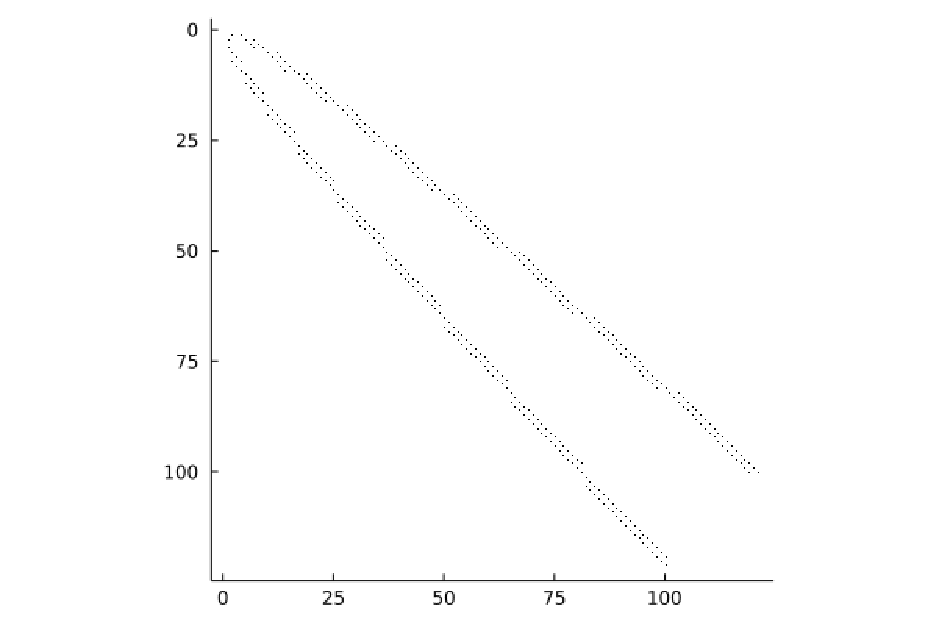
\includegraphics[scale=0.5]{spy-of-Jx}}
		\centering
		\caption{$J_x$}
	\end{subfigure}\hfil % <-- added
	\begin{subfigure}{0.5\textwidth}
		\centerline{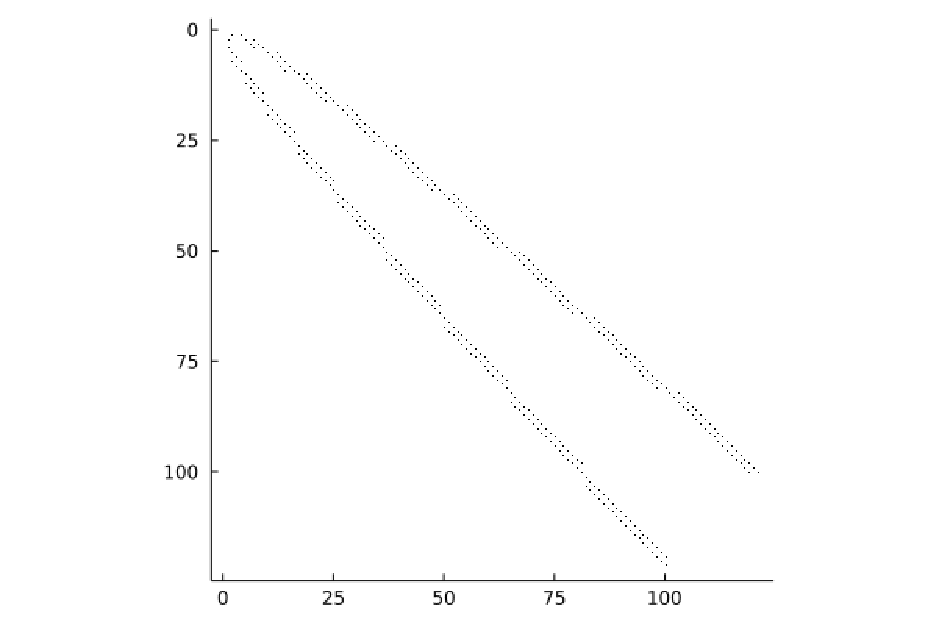
\includegraphics[scale=0.5]{spy-of-Jy}}
		\centering
		\caption{$J_y$}
	\end{subfigure}\hfil % <-- added

	\medskip
	\begin{subfigure}{0.5\textwidth}
		\centerline{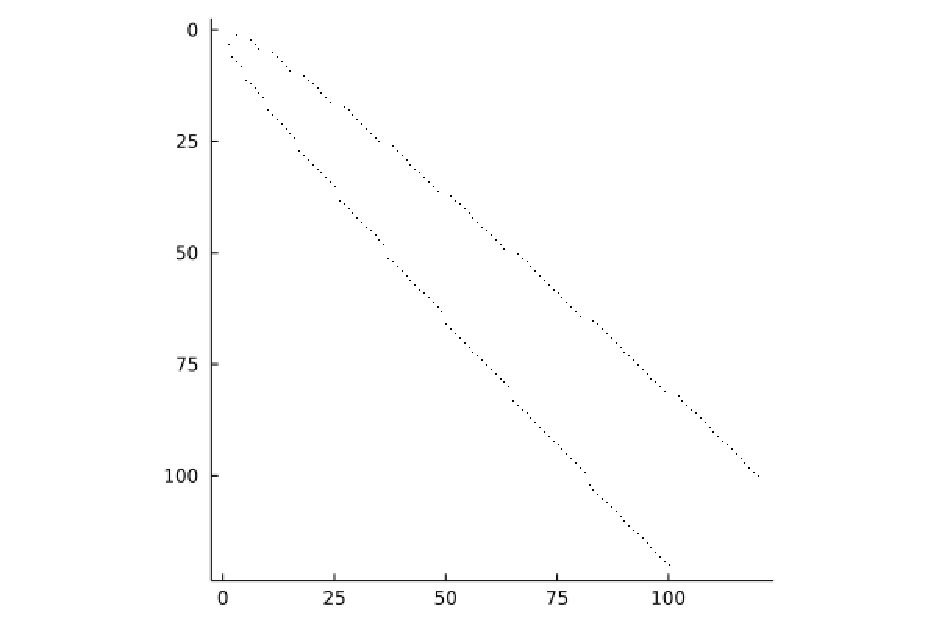
\includegraphics[scale=0.5]{spy-of-Jz}}
		\centering
		\caption{$J_z$}
	\end{subfigure}\hfil % <-- added
	\caption{\enquote{Spy} plots of the Jacobi operator matrices, showing their sparsity and structure, up to order $N=10$. Each are block-tridiagonal, with the blocks corresponding to polynomial degree.}
	\label{fig:sh-spy-jacobi}
\end{figure}

Using \bsrefeqns{eqn:shrecx}{eqn:shrecz}, we have that the Jacobi matrices take the following block-tridiagonal form (i.e. have block-bandwidths $(1,1)$):
\bseqn{
	J_{x/y/z} &= 
		\begin{pmatrix}
			B_{x/y/z,0} & A_{x/y/z,0} & & & & \\
			C_{x/y/z,1} & B_{x/y/z,1} & A_{x/y/z,1} & & & \\
			& C_{x/y/z,2} & B_{x/y/z,2} & A_{x/y/z,2}  & & & \\
			& & C_{x/y/z,3} & \ddots & \ddots & \\
			& & & \ddots & \ddots & \ddots \\
		\end{pmatrix}.
}
$J_x$ has subblock-bandwidths $(2,2)$, where the blocks for \nomenclature[N]{$\N$}{The natural numbers (positive integers)} \nomenclature[N0]{$\No$}{The set $\N \cup \{0\}$} $l \in \No$ are given by:
\bseqn{
	A_{x,l} &:= 
		\begin{pmatrix}
			\alpha_{l,-l,3} & 0 & \alpha_{l,-l,4} & & \\
			& \ddots & \ddots & \ddots & \\
			& & \alpha_{l,l,3} & 0 & \alpha_{l,l,4} \\
		\end{pmatrix} \in \R^{(2l+1)\times(2l+3)}, \\
	B_{x,l} &:= 0 \in \R^{(2l+1)\times(2l+1)} \\
	C_{x,l} &:= 
		\begin{pmatrix}
			\alpha_{l,-l,2} & & \\
			0 & \ddots & \\
			\alpha_{l,-l+2,1} & \ddots & \alpha_{l,l-2,2} \\
			& \ddots & 0 \\
			& & \alpha_{l,l,1}
		\end{pmatrix} \in \R^{(2l+1)\times(2l-1)} \quad (l \ne 0).
}
$J_y$ also has subblock-bandwidths $(2,2)$, where the blocks for $l \in \No$ are given by:
\bseqn{
	A_{y,l} &:= 
		\begin{pmatrix}
			\beta_{l,-l,3} & 0 & \beta_{l,-l,4} & & \\
			& \ddots & \ddots & \ddots & \\
			& & \beta_{l,l,3} & 0 & \beta_{l,l,4} \\
		\end{pmatrix} \in \C^{(2l+1)\times(2l+3)}, \\
	B_{y,l} &:= 0 \in \R^{(2l+1)\times(2l+1)} \\
	C_{y,l} &:= 
		\begin{pmatrix}
			\beta_{l,-l,2} & & \\
			0 & \ddots & \\
			\beta_{l,-l+2,1} & \ddots & \beta_{l,l-2,2} \\
			& \ddots & 0 \\
			& & \beta_{l,l,1}
		\end{pmatrix} \in \C^{(2l+1)\times(2l-1)} \quad (l \ne 0).
}
Finally, $J_z$ has subblock-bandwidths $(1,1)$, where the blocks for $l \in \No$ are given by:
\bseqn{
	A_{z,l} &:= 
		\begin{pmatrix}
			0 & \gamma_{l,-l,2} & 0 & & \\
			& \ddots & \ddots & \ddots & \\
			& & 0 &  \gamma_{l,l,2} & 0 \\
		\end{pmatrix} \in \R^{(2l+1)\times(2l+3)}, \\
	B_{z,l} &:= 0 \in \R^{(2l+1)\times(2l+1)} \\
	C_{z,l} &:= 
		\begin{pmatrix}
			0 & & \\
			\gamma_{l,-l+1,1} & \ddots & \\
			0 & \ddots & 0 \\
			& \ddots & \gamma_{l,l-1,1} \\
			& & 0
		\end{pmatrix} \in \R^{(2l+1)\times(2l-1)} \quad (l \ne 0).
}
The sparsity and structure of the Jacobi matrices as we have defined them can be seen visually in \bsreffig{fig:sh-spy-jacobi}.


\section{Three-term recurrence relation for $\SHvec$}

Three-term recurrence relations for orthogonal polynomials are well established (see for example \cite[Section 18.9]{DLMF}), including for multidimensional OPs \cite[Section 3.2]{dunkl2014orthogonal}. In a similar vein, we can obtain a recurrence relation for the spherical harmonics by combining each system in \bsrefeqn{eqn:jacobimatsdef} in a specific way. It should be emphasised at this point that this is not necessarily the optimal way of computing the spherical harmonics; various efficient methods and algorithms have been proposed (see e.g. \cite{guy1998efficient, sloan2013efficient, fukushima2012numerical}). We present this method in order to be able to generalise it to other multidimensional OP families later on in this thesis.

Rewriting \bsrefeqn{eqn:jacobimatsdef}, we have that: \nomenclature[I]{$I$, $I_d$}{The identity matrix (in $\R^{d \times d}$)}
\bseqn{
	(J_x - xI)\SHvec(x,y,z) = (J_y - yI)\SHvec(x,y,z) = (J_z - zI)\SHvec(x,y,z) = \vec{0}.
}
Combining these relationships into a single system, complete with initial (degree 0) value, results in:
\bseqn{
	\renewcommand\arraystretch{1.3}
	\begin{pmatrix}
		1 & & & \\
		B_0-G_0(x,y,z) & A_0 & & \\
		C_1 & B_1-G_1(x,y,z) & \quad A_1 \quad & \\
		& C_2 & B_2 - G_2(x,y,z)  & \ddots \\
		& & \ddots &\ddots
	\end{pmatrix}
	\SHvec(x,y,z)
	=
	\begin{pmatrix}
		Y_0 \\ 0 \\ 0 \\ 0 \\ \vdots
	\end{pmatrix},
}
where we note $Y_0^0(x,y,z) \equiv Y_0 := c_0^0 \: P_0^{(0,0)} \equiv \half {1 \over \sqrt{\pi}}$, and for each $l = 0,1,2\dots$,
\bseqnnumber{
	A_l &:= 
		\begin{pmatrix}
			A_{x,l} \\
			A_{y,l} \\
			A_{z,l}
		\end{pmatrix} \in \C^{3(2l+1)\times(2l+3)}, \quad
	C_l := 
		\begin{pmatrix}
			C_{x,l} \\
			C_{y,l} \\
			C_{z,l}
		\end{pmatrix} \in \C^{3(2l+1)\times(2l-1)} \quad (n \ne 0), \label{eqn:clenshawmats1} \\
	B_l &:= 
		\begin{pmatrix}
			B_{x,l} \\
			B_{y,l} \\
			B_{z,l}
		\end{pmatrix} \in \C^{3(2l+1)\times(2l+1)}, \quad
	G_n(x,y) := 
		\begin{pmatrix}
			x\idmat{2l+1} \\
			y\idmat{2l+1} \\
			z\idmat{2l+1}
		\end{pmatrix}  \in \C^{3(2l+1)\times(2l+1)}. \label{eqn:clenshawmats2}
}
 
For each $l = 0,1,2\dots$ let $\Dlt$ be any matrix that is a left inverse of $A_l$, i.e. such that $\Dlt A_l = \idmat{2l+3}$. Multiplying our system by the preconditioner matrix that is given by the block diagonal matrix of the $\Dlt$'s, we obtain a lower triangular system \cite[Section 3.2]{dunkl2014orthogonal}, which can be expanded to obtain the three-term recurrence, for $l = 0,1,2,\dots$:
\bseqn{
	\begin{cases}
		\SHvec_{-1}(x,y,z) := 0 \\
		\SHvec_{0}(x,y,z) := Y_0 \\
		\SHvec_{l+1}(x,y,z) = -\Dlt (B_l-G_l(x,y,z)) \SHvec_l(x,y,z) - \Dlt C_l  \,\SHvec_{l-1}(x,y,z)
	\end{cases}
}

Since the above holds for any $\Dlt$ that is a left inverse of $A_l$, we are free to choose the $\Dlt$ matrices in the following way. For $l \in \N$, we can set
\bseqnnumber{
	\Dlt = 
		\begin{pmatrix}
			& & & & & \vec{\eta}^\top_{0} \\
			0 & & & 0 & & & {1 \over \gamma_{l,-l,2}} & \\
			& \ddots & & & \ddots & & & \ddots \\
			& & 0 & & & 0 & & & {1 \over \gamma_{l,l,2}} \\
			& & & & & \vec{\eta}^\top_{1} 
		\end{pmatrix} \in \R^{(2n+3)\times3(2n+1)}, \label{eqn:Dltdef}
}
where $\vec{\eta}_{0}, \vec{\eta}_{1} \in \R^{3(2n+1)}$ are vectors with entries given by 
\bseqn{
	\big(\vec{\eta}_{0}\big)_j &= 
		\begin{cases}
			{1 \over \alpha_{l,-l,3}} & j = 1 \\
			{- \; \alpha_{l,-l,4} \over \alpha_{l,-l,3} \: \gamma_{l,1-l,2}} & j = 2(2n+1) + 2 \\
			0 & o/w
		\end{cases}, \\
	\big(\vec{\eta}_{1}\big)_j &= 
		\begin{cases}
			{1 \over \alpha_{l,l,4}} & j = 2l+1 \\
			{- \; \alpha_{l,l,3} \over \alpha_{l,l,4} \: \gamma_{l,l-1,2}} & j = 3(2n+1) - 1 \\
			0 & o/w
		\end{cases}.
}
For $l = 0$ we can simply set
\bseqnnumber{
	D^T_0 = 
		\begin{pmatrix}
			{\beta_{0,0,4} \over \alpha_{0,0,3} \beta_{0,0,4} - \alpha_{0,0,4} \beta_{0,0,3}} & {- \alpha_{0,0,4} \over \alpha_{0,0,3} \beta_{0,0,4} - \alpha_{0,0,4} \beta_{0,0,3}} & 0 \\
			0 & 0 & {1 \over \gamma_{0,0,2}} \\
			{\beta_{0,0,3} \over \alpha_{0,0,4} \beta_{0,0,3} - \alpha_{0,0,3} \beta_{0,0,4}} & {- \alpha_{0,0,3} \over \alpha_{0,0,4} \beta_{0,0,3} - \alpha_{0,0,3} \beta_{0,0,4}} & 0
		\end{pmatrix}. \label{eqn:Dzerotdef}
}
It will be convenient for us to give a formal name for these coefficient matrices above for a family of multidimensional orthogonal polynomials.
\begin{definition}\label{def:clenshawmats}
	The matrices $-\Dlt (B_l-G_l(x,y,z))$, $\Dlt C_l$ for $l \in \No$ defined via \bsrefeqns{eqn:clenshawmats1}{eqn:Dzerotdef} are called the recurrence coefficient matrices for a given family of multidimensional orthogonal polynomials.
\end{definition}



\section{Computational aspects}

Once again, let $f(x,y,z)$ be a function on the unit sphere $\Omega$ be approximated by its expansion 
\bseqn{
	f(x,y,z) \approx \SHvec(x,y,z)^\top \fvec = \sum^N_{l=0} \SHvecl(x,y,z)^\top \fvec_l =  \sum^N_{l=0}  \sum^l_{m=-l} f_{l,m} \: \Ylmxyz,
}
where $\SHvecl (x,y,z), \fvec_l \in \C^{2l+1}$ for each $l \in \{0,\dots,N\}$, for some coefficients vector $\fvec = (f_{l,m})$ up to degree order $N \in \N$.


\subsection{Obtaining coefficients}

In spectral space, we wish to work only with vectors of coefficients for the expansion of a function, to which we can apply operator matrices to that represent differential or other operations. Naturally, we of course need a way to obtain the coefficients $f_{l,m}$. The coefficients can be calculated via the integral
\bseqn{
	f_{l,m} = \int_\Omega f(\costheta \sinphi, \sintheta \sinphi, \cosphi) \: \Ylmfull^* \: \sinphi \: \D \varphi \: \D \theta
}
using the orthonormality of the spherical harmonics. As discussed in \bsrefchapter{CHAPTER:intro}, methods to calculate these coefficients exist known as spectral transforms, and are well established for the spherical harmonics (see e.g. \cite{mohlenkamp1999fast, suda2002fast}). Additionally, packages are available for public use that implement efficient spherical harmonics transforms, for example the FastTransforms package \cite{slevinsky2019fast}.


\subsection{Function evaluation}\label{subsubsection:clenshaw}

A multivariate analogue of Clenshaw's recursive algorithm for evaluation of a function expanded in an OP basis has been established for methods on other domains in 2D such as the triangle \cite{olver2019triangle}, and we proceed similarly here. We can use the Clenshaw algorithm to evaluate this function at a given point $(x,y,z)$ on $\Omega$ \cite{press2007numerical}. The multidimensional \textit{Clenshaw algorithm} is as follows:
\bseqn{
	\quad &\text{1) } \text{Set } \vec{\xi}_{N+2} = \bold{0}, \: \vec{\xi}_{N+2} = \bold{0}. \\
	\quad &\text{2) } \text{For } n = N:-1:0 \\
	\quad & \quad \quad \quad \text{set } \vec{\xi}_{n}^T = \fvec_n^T - \vec{\xi}_{n+1}^T D^T_n (B_n - G_n(x,y,z)) -  \vec{\xi}_{n+2}^T D^T_{n+1}C_{n+1} \\
	\quad &\text{3) } \text{Output: } f(x,y,z) \approx \vec{\xi}_{0}^T \SHvec_0(x,y,z) \equiv \xi_0 Y_0.
}


\subsection{Obtaining operator matrices for variable coefficients}

The Clenshaw algorithm presented in \bsrefsection{subsubsection:clenshaw} can also be used with the Jacobi matrices replacing the point $(x,y,z)$, to yield an operator matrix. 

Let us explain what we mean by this. Suppose $v : \Omega \to \C$ is a function, and we encounter the problem of finding the coefficients of the expansion for $v(x,y,z) f(x,y,z)$. We wish to therefore find an operator $V$ for $v$ so that
\bseqn{
	v(x,y,z) f(x,y,z) = v(x,y,z) \fvec^\top \SHvec(x,y,z) = (V \fvec)^\top \SHvec(x,y,z),
}
i.e. $V \fvec$ is the coefficients vector for the expansion of the function $(x,y,z) \mapsto v(x,y,z) f(x,y,z)$ in the spherical harmonic basis.

Let $\vec{v}$ be the coefficients of the expansion of $v$ up to order $N$. The operator $V$ would then be the result of the following \textit{operator Clenshaw algorithm}:
\bseqn{
	\quad &\text{1) } \text{Set } \vec{\xi}_{N+2} = \bold{0}, \: \vec{\xi}_{N+2} = \bold{0}. \\
	\quad &\text{2) } \text{For } n = N:-1:0 \\
	\quad & \quad \quad \quad \text{set } \vec{\xi}_{n}^T = \vec{v}_n^T - \vec{\xi}_{n+1}^T D^T_n (B_n - G_n(J_x,J_y,J_z)) -  \vec{\xi}_{n+2}^T D^T_{n+1}C_{n+1} \\
	\quad &\text{3) } \text{Output: } f(x,y,z) \approx \vec{\xi}_{0}^T \SHvec_0(x,y,z) \equiv \xi_0 Y_0
}
where at each iteration, $\vec{\xi}_n$ is a vector of matrices (note that we are abusing notation here a bit, however it is the simplest way to present the algorithm without introducing yet more matrices!).





%%% TANGENT BUNDLE ----- VECTOR SHs
\section{Vector spherical harmonics as orthogonal vectors in three variables}\label{section:VSHs}

We have established that the spherical harmonics can be viewed as a basis of orthonormal polynomials on the sphere. Specifically, given a function $f : \Omega \to \C$, we can write $f = \sum_{l = 0}^{N} \sum_{m = -l}^{l} f_{l,m} \; \Ylm$ where $\{f_{l,m}\}$ are coefficients and $N \in \N$ is sufficiently large. But what about vector-valued functions? \nomenclature[r]{$\rvec$}{The unit normal vector at the point $(x,y,z)$}
\begin{definition}\label{def:tangentbundle}
	Let $(x,y,z) \in \Omega$. We refer to the \textbf{tangent space} of the point $(x,y,z)$ as the space of all vectors that are orthogonal to the vector $\rvec := [x,y,x]^\top$. We further define the \textbf{tangent bundle} of $\Omega$ as the set of all such spaces for every point in $\Omega$.
\end{definition}
For the purposes of this discussion, we will only consider the tangent bundle, and thus wish to write down a basis for vector-valued functions with values in the tangent bundle. Fortunately, there is a simple solution known as the \textit{vector spherical harmonics (VSHs)} \cite{barrera1985vector}: \nomenclature[grad]{$\gradS$}{The spherical gradient operator} \nomenclature[Psilm]{$\gradYlm$}{The vector spherical harmonic $\gradS \Ylm$} \nomenclature[Philm]{$\gradpYlm$}{The vector spherical harmonic $\gradS^\perp \Ylm = \rvec \times \gradS \Ylm$}
\bseqnnumber{
	\gradYlm &:= \gradS \Ylm = \ppx{\phi} \Ylm \phivec + {1 \over \sinphi} \ppx{\theta} \Ylm \thetavec, \nonumber \\
	\gradpYlm &:= \gradS^\perp \Ylm \equiv \rvec \times \gradS \Ylm = \ppx{\phi} \Ylm \thetavec - {1 \over \sinphi} \ppx{\theta} \Ylm \phivec. \label{eqn:VSHs}
}
Here, $\rvec$ is simply the outward unit normal vector to the surface of the sphere at the point $(x,y,z)$, while \nomenclature[phi theta vector]{$\phivec$, $\thetavec$}{The standard spherical coordinate angular basis vectors} $\phivec, \thetavec$ are the standard spherical coordinate unit vectors, i.e. $\phivec := [\costheta \cosphi, \sintheta \cosphi, -\sinphi]^\top$, $\thetavec := [-\sintheta, \costheta, 0]^\top$. They are orthogonal with respect to the inner product \nomenclature[inner]{$\ip<u, v>$}{An inner product (defined by the context)}  $\ip<\vec{A}, \vec{B}> = \iint_\Omega \vec{A} \cdot \vec{B}^* \: \sinphi \: \D\varphi \: \D\theta$ -- in particular, for any $l, l' \in \N$, $m, m' \in \Z$ s.t. $-l \le m \le l$, $-l' \le m' \le l'$,
\bseqn{
	\ip<\gradYlm, \gradYlmprime> &= \iint_\Omega \gradYlm \cdot {\gradYlmprime}^* \: \sinphi \: \D\varphi \: \D\theta = \delta_{l,l'} \delta_{m,m'} \: l (l+1), \\
	\ip<\gradpYlm, \gradpYlmprime> &= \iint_\Omega \gradpYlm \cdot {\gradpYlmprime}^* \: \sinphi \: \D\varphi \: \D\theta = \delta_{l,l'} \delta_{m,m'} \: l (l+1), \\
	\ip<\gradYlm, \gradpYlmprime> &= \iint_\Omega \gradpYlm \cdot {\gradpYlmprime}^* \: \sinphi \: \D\varphi \: \D\theta = 0.
} 
Let $\uvec$ be a vector-valued function on $\Omega$ whose values are of the form
\bseqn{
	\uvec(x,y,z) = u_\varphi(x,y,z) \: \phivec + u_\theta(x,y,z) \: \thetavec, \quad (x,y,z) \in \Omega
}
for some scalar functions $u^\varphi, u^\theta$. Such a function $\uvec$ we refer to as a \textit{vector-valued function in the tangent bundle} of the sphere. Importantly, the set $\{\gradYlm, \gradpYlm\}$ form a complete and orthogonal basis for such functions \cite{barrera1985vector}. That is, given $\uvec$, there exist coefficients $\{u_{l,m}^{\gradYlm}, u_{l,m}^{\gradpYlm} \}$ such that for large enough $N$:
\bseqn{
	\uvec = \sum_{l = 0}^{N} \sum_{m = -l}^{l} u_{l,m}^{\gradY} \; \gradYlm + u_{l,m}^{\gradpY} \; \gradpYlm.
}
Vector spherical harmonics have been widely used in electrostatics (e.g. \cite{barrera1985vector}), electrodynamics (e.g. \cite{carrascal1991vector}), and of course fluid dynamics including weather and climate modelling (e.g. \cite{moses1974use, fengler2005nonlinear, swarztrauber1996spectral}). Other definitions for VSHs are used (e.g. \cite{hill1954theory}), however it is convenient for deriving explicit sparse relations and operators to use the ones described here. In particular, we can note that computing the gradient or divergence of a function is merely a matter of conversion between the SH and the VSH bases.

A simple calculation shows that such orthogonal vectors must still have block-tridiagonal Jacobi operators, as multiplication by $x, y$, or $z$ remains inside the ideal. Thus, we we can use the same techniques that we used for the scalar SHs to derive Jacobi matrices, function evaluation and transforms.


\subsection{Jacobi matrices}

We start as before for the scalar case by finding $x \, \gradYlm (x,y,z)$, $y \,\gradYlm (x,y,z)$, $z \, \gradYlm (x,y,z)$, and $x \,\gradpYlm (x,y,z)$, $y \, \gradpYlm (x,y,z)$, $z \,\gradpYlm (x,y,z)$ in terms of $\gradYlmprime (x,y,z)$, $\gradpYlmprime (x,y,z)$. A lovely consequence of our definitions of the scalar and vector spherical harmonics is that we can once again find explicit expressions for the coefficients in the aforementioned relations. To this end, we recall and derive some important relations of the complex exponential and Jacobi polynomials that are a part of the spherical harmonics definitions. In particular we first note that:
\bseqnnumber{
	\int_0^{2\pi} \: \eimtheta \: e^{-im'\theta} \: \cos(\theta) \D\theta &= \pi (\delta_{m',m-1} + \delta_{m',m+1}) \label{eqn:intcomplexexpcos} \\
	\int_0^{2\pi} \: \eimtheta \: e^{-im'\theta} \: \sin(\theta) \D\theta &= i \; \pi (\delta_{m',m-1} - \delta_{m',m+1}) \label{eqn:intcomplexexpsin}
}
and, for $l \in \No, m \in \Z$ s.t. $-l \le m \le l$,
\bseqnnumber{
	&\int_{-1}^1 \: \jaclmabs{l}{m}(z) \: \jaclmabs{l'}{m}(z) \: \rho(z)^{2\abs{m}} \: \D z = \delta_{l',l} \: {1 \over 2\pi (\clm)^2} \label{eqn:normjac} \\
	&\jaclmabsdz{l}{m}(z) = d_{l,m} \: \jaclmbracket{l}{\abs{m} + 1} \quad \text{where } 
	d_{l,m} := 
		\begin{cases}
			\half (l + \abs{m} + 1) & l > \abs{m} \\
			0 & l = \abs{m}
		\end{cases}. \label{eqn:diffjac}
}
\bsrefeqncapital{eqn:normjac} and \bsrefeqn{eqn:diffjac} are simply consequences of the definition of the Jacobi polynomials -- see \cite[Table 18.3.1]{DLMF} and \cite[18.9.15]{DLMF}. 

The expressions for the VSHs as given in \bsrefeqn{eqn:VSHs} together with the above allow us to be able to find the coefficients for our desired expressions for $x \gradYlm$, $y \gradYlm$, $z \gradYlm$, $x \gradpYlm$, $y \gradpYlm$ and $z \gradpYlm$. 

\begin{lemma}\label{lemma:VSHrecurrences}
	For $l \in \N$ and $m \in \Z$ s.t. $-l \le m \le l$, the vector spherical harmonics satisfy the relationships: \nomenclature[Alpha]{$A_{l,m,j}$}{Capital greek letters with subscripts refer to coefficients in vector OP (VSH) relations (unless otherwise stated)}
\bseqn{
	x \gradYlm &= A_{l,m,1} \gradY^{m-1}_{l-1} + A_{l,m,2} \gradY^{m+1}_{l-1} + A_{l,m,3} \gradY^{m-1}_{l+1} + A_{l,m,4} \gradY^{m+1}_{l+1} \\
& \quad \quad \quad + A_{l,m,5} \gradpY^{m-1}_{l} + A_{l,m,6} \gradpY^{m+1}_{l}, \\
	x \gradpYlm &= A_{l,m,1} \gradpY^{m-1}_{l-1} + A_{l,m,2} \gradpY^{m+1}_{l-1} + A_{l,m,3} \gradpY^{m-1}_{l+1} + A_{l,m,4} \gradpY^{m+1}_{l+1} \\
& \quad \quad \quad - A_{l,m,5} \gradY^{m-1}_{l} - A_{l,m,6} \gradY^{m+1}_{l}, \\
	y \gradYlm &= B_{l,m,1} \gradY^{m-1}_{l-1} + B_{l,m,2} \gradY^{m+1}_{l-1} + B_{l,m,3} \gradY^{m-1}_{l+1} + B_{l,m,4} \gradY^{m+1}_{l+1} \\
& \quad \quad \quad + B_{l,m,5} \gradpY^{m-1}_{l} + B_{l,m,6} \gradpY^{m+1}_{l}, \\
	y \gradpYlm &= B_{l,m,1} \gradpY^{m-1}_{l-1} + B_{l,m,2} \gradpY^{m+1}_{l-1} + B_{l,m,3} \gradpY^{m-1}_{l+1} + B_{l,m,4} \gradpY^{m+1}_{l+1} \\
& \quad \quad \quad - B_{l,m,5} \gradY^{m-1}_{l} - B_{l,m,6} \gradY^{m+1}_{l}, \\
	z \gradYlm &= \Gamma_{l,m,1} \gradY^{m}_{l-1} + \Gamma_{l,m,2} \gradY^{m}_{l+1} + \Gamma_{l,m,3} \gradpY^{m}_{l}, \\
	z \gradpYlm &= \Gamma_{l,m,1} \gradpY^{m}_{l-1} + \Gamma_{l,m,2} \gradpY^{m}_{l+1} - \Gamma_{l,m,3} \gradY^{m}_{l}
}
where,
\bseqn{
	A_{l,m,1} &:= {\clm c_{l-1}^{m-1} \over 2 l (l-1)}
		\begin{cases}
			\tilde A_{l,m,1} & \text{if } m > 0 \\
			\tilde A_{l,\abs{m},2} & \text{if } m \le 0
		\end{cases} \\
	A_{l,m,2} &:= {\clm c_{l-1}^{m+1} \over 2 l (l-1)}
		\begin{cases}
			\tilde A_{l,m,2} & \text{if } m \ge 0 \\
			\tilde A_{l,\abs{m},1} & \text{if } m < 0
		\end{cases} \\
	A_{l,m,3} &:= {\clm c_{l+1}^{m-1} \over 2 (l+1)(l+2)}
		\begin{cases}
			\tilde A_{l,m,3} &\text{if } m > 0 \\
			\tilde A_{l,\abs{m},4} &\text{if } m \le 0
		\end{cases} \\
	A_{l,m,4} &:= {\clm c_{l+1}^{m+1} \over 2 (l+1)(l+2)}
		\begin{cases}
			\tilde A_{l,m,4} &\text{if } m \ge 0 \\
			\tilde A_{l,\abs{m},3} &\text{if } m < 0
		\end{cases} \\
	A_{l,m,5} &:= {i \over 2l(l+1)}
		\begin{cases}
			- i \: d_{l,m - 1} \: {c_l^{m-1} \over 2 \clm} &\text{if } m > 0 \\
			i \: d_{l,\abs{m}} \: {\clm \over 2 c_l^{m-1}} &\text{if } m \le 0
		\end{cases} \\
	A_{l,m,6} &:= {i \over 2l(l+1)}
		\begin{cases}
			- d_{l,m} \: {\clm \over c_l^{m+1}} &\text{if } m \ge 0 \\
			d_{l,\abs{m} - 1} \: {c_l^{m+1} \over \clm} &\text{if } m < 0
		\end{cases} \\
	B_{l,m,j} &:= i (-1)^{j+1} A_{l,m,j} \quad \text{for } j = 1,\dots,6 \\
	\Gamma_{l,m,1} &:= {\clm c_{l-1}^{m} \over l(l-1)} \Big[ \abs{m}(\abs{m} + 2) {\tilde \gamma_{l,\abs{m},1} \over (c_{l-1}^{\abs{m}})^2} + d_{l,\abs{m}} d_{l-1,\abs{m}} {\tilde \gamma_{l,\abs{m}+1,1} \over (c_{l-1}^{\abs{m}+1})^2} \Big] \\
	\Gamma_{l,m,2} &:= {\clm c_{l+1}^{m} \over (l+1)(l+2)} \Big[ \abs{m}(\abs{m} + 2) {\tilde \gamma_{l,\abs{m},2} \over (c_{l+1}^{\abs{m}})^2} + d_{l,\abs{m}} d_{l+1,\abs{m}} {\tilde \gamma_{l,\abs{m}+1,2} \over (c_{l+1}^{\abs{m}+1})^2} \Big] \\
	\Gamma_{l,m,3} &:= {i \: m \over l(l+1)}
}
where the $c_{l'}^{m'}$, $d_{l',m'}$, $\tilde \gamma_{l',m',j}$ are defined in \bsrefeqn{eqn:clmdef}, \bsrefeqn{eqn:diffjac} and \bsrefcor{corollary:jacobirelations} respectively, and
\bseqn{
	\tilde A_{l,m,1} &:= \Big( (m^2 - 1) \tilde \alpha_{l-1,m-1,4} - d_{l-1,m-1} \tilde \gamma_{l-1,m,2} \Big) {1 \over (\clm)^2} + d_{l,m} d_{l-1,m-1} {\tilde \alpha_{l,m+1,1} \over (c_{l-1}^{m})^2} \\
	\tilde A_{l,m,2} &:= \Big( m(m+2) \tilde \alpha_{l,m,2} - d_{l,m} \tilde \gamma_{l,m+1,1} \Big) {1 \over (c_{l-1}^{m+1})^2} + d_{l,m} d_{l-1,m+1} {\tilde \alpha_{l-1,m+2,3} \over (c_{l}^{m+1})^2} \\
	\tilde A_{l,m,3} &:= \Big( (m^2 - 1) \tilde \alpha_{l+1,m-1,2} - d_{l+1,m-1} \tilde \gamma_{l+1,m,1} \Big) {1 \over (\clm)^2} + d_{l,m} d_{l+1,m-1} {\tilde \alpha_{l,m+1,3} \over (c_{l+1}^{m})^2} \\
	\tilde A_{l,m,4} &:= \Big( m(m+2) \tilde \alpha_{l,m,4} - d_{l,m} \tilde \gamma_{l,m+1,2} \Big) {1 \over (c_{l+1}^{m+1})^2} + d_{l,m} d_{l+1,m+1} {\tilde \alpha_{l+1,m+2,1} \over (c_{l}^{m+1})^2}.
}
where again the $\tilde \alpha_{l',m',j}$ are defined in \bsrefcor{corollary:jacobirelations} too.
\end{lemma}

\remark We emphasise again that it is due to the unique relationships that the Jacobi polynomials possess that we are able to explicitly write down these coefficients.

\begin{proof}[Proof of \bsreflemma{lemma:VSHrecurrences}]

	Fix $l \in \N$ and $m \in \Z$ s.t. $-l \le m \le l$. The proof we will use is to directly calculate the nonzero coefficients in each expansion using inner products. To this end, note that
\bseqn{
	x \gradYlm = \sum_{l'=1}^{l+1} \sum_{m'=-l'}^{l'} \calA_{l',m'} \gradYlmprime + \calA^\perp_{l',m'} \gradpYlmprime
}
where the coefficients are given by
\bseqn{
	\calA_{l',m'} = {\ip<x \gradYlm, \gradYlmprime> \over \norm{\gradYlmprime}^2} = {1 \over l'(l'+1)} \ip<x \gradYlm, \gradYlmprime> \\
	\calA^\perp_{l',m'} = {\ip<x \gradYlm, \gradpYlmprime> \over \norm{\gradpYlmprime}^2} = {1 \over l'(l'+1)} \ip<x \gradYlm, \gradpYlmprime>.
}
The aim will be to show that the only nonzero coefficients $\calA_{l',m'}$, $\calA^\perp_{l',m'}$ match the $A_{l,m,j}$ for $j=1,\dots,6$ in the Lemma. Now, using a change of variable, we have that
\bseqnnumber{
	&\ip<x \gradYlm, \gradYlmprime> \nonumber \\
	&= \iint_\Omega \costheta \sinphi \: \gradYlm \cdot {\gradYlmprime}^* \sinphi \: \D\phi \: \D\theta \nonumber \\
	&= \clm \clmprime \Big( \int_0^{2\pi} \eimtheta \eimthetaprime \costheta \: \D\theta \Big) \nonumber \\
	&\quadfour \cdot \Big( \int_{-1}^{1} \Big\{ \big[ \abs{m} z \jaclmabs{l}{m}(z) - \rho(z)^2 \jaclmabsdz{l}{m}(z) \big] \nonumber \\
	&\quadeight \quadtwo \cdot \big[ \abs{m'} z \jaclmabs{l'}{m'}(z) - \rho(z)^2 \jaclmabs{l'}{m'}(z) \big] \nonumber \\
	&\quadeight + mm' \jaclmabs{l}{m}(z) \jaclmabs{l'}{m'}(z) \Big\} \: \rho(z)^{\abs{m}+\abs{m'}-1} \: \D z \Big) \nonumber \\
	&= \clm \clmprime \pi (\delta_{m',m-1} + \delta_{m',m+1}) \nonumber \\
	&\quadfour \cdot \Big( \int_{-1}^{1} \Big\{ \jaclmabs{l}{m} \jaclmabs{l'}{m'} \rho^{\abs{m}+\abs{m'}-1} \big(mm' + \abs{m}\abs{m'} z^2 \big) \nonumber \\
	&\quadeight - \abs{m} z \jaclmabs{l}{m} \jaclmabsdz{l'}{m'} \rho^{\abs{m}+\abs{m'}+1} \nonumber \\
	&\quadeight - \abs{m'} z \jaclmabsdz{l}{m} \jaclmabs{l'}{m'} \rho^{\abs{m}+\abs{m'}+1} \nonumber  \\
	&\quadeight + \jaclmabsdz{l}{m} \jaclmabsdz{l'}{m'} \rho^{\abs{m}+\abs{m'}+3} \Big\} \: \D z \Big). \label{eqn:lemmaVSHrecurrencesproof}
}
We can conclude that the only possible nonzero coefficients are when $m' = m \pm 1$, and so it is left to evaluate the integral that is left at \bsrefeqn{eqn:lemmaVSHrecurrencesproof} when $m'$ takes either value. Since we need to take account of the fact that $m$ can be negative, to simplify our argument we make use of the fact that $m' = m - 1$ for $m < 0$ is analogous to the case $m' = m+1$ for $m > 0$, and vice versa. 

On that note, we will first consider the case that $m > 0$ and $m' = m - 1$, and calculate the integral in \bsrefeqn{eqn:lemmaVSHrecurrencesproof}:
\bseqnnumber{
	&\int_{-1}^{1} \Big\{ m(m-1) \jaclm{l}{m} \jaclmbracket{l'}{m-1} \rho^{2m-2} (1 + z^2) - m z \jaclm{l}{m} \jaclmbracketdz{l'}{m-1} \rho^{2m} \nonumber \\
	&\quadtwo \quad - (m-1) z \jaclmdz{l}{m} \jaclmbracket{l'}{m-1} \rho^{2m} + \jaclmdz{l}{m} \jaclmbracketdz{l'}{m-1} \rho^{2m+2} \Big\} \: \D z \nonumber \\
	&= \int_{-1}^{1} \Big\{ m(m-1) \jaclm{l}{m} \jaclmbracket{l'}{m-1} \rho^{2m-2} (1 + z^2) - m z \jaclm{l}{m} \jaclmbracketdz{l'}{m-1} \rho^{2m} \nonumber \\
	&\quadtwo + (m-1) \jaclm{l}{m} \rho^{2m-2} \big(\jaclmbracket{l'}{m-1} \rho^{2} - z \jaclmbracketdz{l'}{m-1} \rho^{2} - 2m z^2 \jaclmbracket{l'}{m-1} \big) \nonumber \\
	&\quadtwo + \jaclmdz{l}{m} \jaclmbracketdz{l'}{m-1} \rho^{2m+2} \Big\} \: \D z \nonumber \\
	&= \int_{-1}^{1} \Big\{ (m-1)(m+1) \jaclm{l}{m} \jaclmbracket{l'}{m-1} \rho^{2m} - z \jaclm{l}{m} \jaclmbracketdz{l'}{m-1} \rho^{2m} \nonumber \\
	&\quadfour + \jaclmdz{l}{m} \jaclmbracketdz{l'}{m-1} \rho^{2m+2} \Big\} \: \D z \nonumber \\
	&= \int_{-1}^{1} \Big\{ (m-1)(m+1) \jaclm{l}{m} \jaclmbracket{l'}{m-1} \rho^{2m} - d_{l',m-1} z \jaclm{l}{m} \jaclm{l'}{m} \rho^{2m} \nonumber \\
	&\quadfour + d_{l,m} d_{l',m-1} \jaclmbracket{l}{m+1} \jaclm{l'}{m} \rho^{2m+2} \Big\} \: \D z \nonumber \\
	&= \int_{-1}^{1} \Big\{ (m^2 - 1) \jaclm{l}{m} \big( \tilde \alpha_{l', m-1, 2} \jaclm{l'-1}{m} + \tilde \alpha_{l', m-1, 4} \jaclm{l'+1}{m} \big) \rho^{2m} \nonumber \\
	&\quadfour - d_{l',m-1} \jaclm{l}{m} \big( \tilde \gamma_{l',m,1} \jaclm{l'-1}{m} + \tilde \gamma_{l',m,2} \jaclm{l'+1}{m} \big) \rho^{2m} \nonumber \\
	&\quadfour + d_{l,m} d_{l',m-1} \jaclm{l'}{m} \big( \tilde \alpha_{l, m+1, 1} \jaclm{l-1}{m} + \tilde \alpha_{l, m+1, 3} \jaclm{l+1}{m} \big) \rho^{2m} \Big\} \: \D z \nonumber \\
	&= {\delta_{l',l-1} \over 2\pi} \Big\{ \big[ (m^2 - 1) \tilde \alpha_{l-1, m-1, 4} - d_{l-1,m-1} \tilde \gamma_{l-1,m,2} \big] {1 \over (\clm)^2} + d_{l,m} d_{l-1,m-1} {\tilde \alpha_{l-1, m-1, 1} \over (c_{l-1}^m)^2} \Big\} \nonumber \\
	&\quadtwo + {\delta_{l',l+1} \over 2\pi} \Big\{ \big[ (m^2 - 1) \tilde \alpha_{l+1, m-1, 2} - d_{l+1,m-1} \tilde \gamma_{l+1,m,1} \big] {1 \over (\clm)^2} \nonumber \\
	&\quadeight + d_{l,m} d_{l+1,m-1} {\tilde \alpha_{l-1, m-1, 3} \over (c_{l+1}^m)^2} \Big\}. \label{eqn:lemmaVSHrecurrencesproof2}
}
As we can see, the coefficients are then also only possibly nonzero for $l' = l \pm 1$. Combining the above with the \bsrefeqn{eqn:lemmaVSHrecurrencesproof}, we have that our two coefficients for $\calA_{l-1,m-1}, \calA_{l+1,m-1}$ are those stated in the Lemma as $A_{l,m,1}$ and $A_{l,m,3}$, for $m > 0$. 

Next, assume $m \ge 0$ and consider the case $m' = m + 1$. The integral in \bsrefeqn{eqn:lemmaVSHrecurrencesproof} is then:
\bseqnnumber{
	&\int_{-1}^{1} \Big\{ m(m+1) \jaclm{l}{m} \jaclmbracket{l'}{m+1} \rho^{2m} (1 + z^2) - m z \jaclm{l}{m} \jaclmbracketdz{l'}{m+1} \rho^{2m+2} \nonumber \\
	&\quadtwo \quad - (m+1) z \jaclmdz{l}{m} \jaclmbracket{l'}{m+1} \rho^{2m+2} + \jaclmdz{l}{m} \jaclmbracketdz{l'}{m+1} \rho^{2m+4} \Big\} \: \D z \nonumber \\
	&= \int_{-1}^{1} \Big\{ m(m+1) \jaclm{l}{m} \jaclmbracket{l'}{m+1} \rho^{2m} (1 + z^2) \nonumber \\
	&\quadfour - (m+1) z \jaclmdz{l}{m} \jaclmbracket{l'}{m+1} \rho^{2m+2} \nonumber \\
	&\quadfour + m \jaclmbracket{l'}{m+1} \rho^{2m} \big( - 2(m+1) z^2 \jaclm{l}{m} + \jaclm{l}{m} \rho^{2} - z \jaclmdz{l}{m} \rho^{2} \big) \nonumber \\
	&\quadfour + \jaclmdz{l}{m} \jaclmbracketdz{l'}{m+1} \rho^{2m+2} \Big\} \: \D z \nonumber \\
	&= \int_{-1}^{1} \Big\{ m(m+2) \jaclm{l}{m} \jaclmbracket{l'}{m+1} \rho^{2m+2} - z \jaclmdz{l}{m} \jaclmbracket{l'}{m+1} \rho^{2m+2} \nonumber \\
	&\quadfour + \jaclmdz{l}{m} \jaclmbracketdz{l'}{m+1} \rho^{2m+4} \Big\} \: \D z \nonumber \\
	&= \int_{-1}^{1} \Big\{ m(m+2) \jaclm{l}{m} \jaclmbracket{l'}{m+1} \rho^{2m+2} - d_{l,m} z \jaclmbracket{l}{m+1} \jaclmbracket{l'}{m+1} \rho^{2m+2} \nonumber \\
	&\quadfour + d_{l,m} d_{l',m+1} \jaclmbracket{l}{m+1} \jaclmbracket{l'}{m+2} \rho^{2m+4} \Big\} \: \D z \nonumber \\
	&= \int_{-1}^{1} \Big\{ m(m+2) \jaclmbracket{l'}{m+1} \big( \tilde \alpha_{l, m, 2} \jaclmbracket{l-1}{m+1} + \tilde \alpha_{l, m, 4} \jaclmbracket{l+1}{m+1} \big) \rho^{2m+2} \nonumber \\
	&\quadtwo - d_{l,m} \jaclmbracket{l'}{m+1} \big( \tilde \gamma_{l,m+1,1} \jaclmbracket{l-1}{m+1} + \tilde \gamma_{l,m+1,2} \jaclmbracket{l+1}{m+1} \big) \rho^{2m+2} \nonumber \\
	&\quadtwo + d_{l,m} d_{l',m+1} \jaclmbracket{l}{m+1} \big( \tilde \alpha_{l', m+2, 1} \jaclmbracket{l'-1}{m+1} + \tilde \alpha_{l', m+2, 3} \jaclmbracket{l'+1}{m+1}  \big) \rho^{2m+2} \Big\} \: \D z \nonumber \\
	&= {\delta_{l',l-1} \over 2\pi} \Big\{ \big[ m(m+2) \tilde \alpha_{l, m, 2} - d_{l,m} \tilde \gamma_{l,m+1,1} \big] {1 \over (c_{l-1}^{m+1})^2} + d_{l,m} d_{l-1,m+1} {\tilde \alpha_{l-1, m+2, 3} \over (c_{l}^{m+1})^2} \Big\} \nonumber \\
	&\quadtwo + {\delta_{l',l+1} \over 2\pi} \Big\{ \big[ m(m+2) \tilde \alpha_{l, m, 4} - d_{l,m} \tilde \gamma_{l,m+1,2} \big] {1 \over (c_{l-1}^{m+1})^2} + d_{l,m} d_{l+1,m+1} {\tilde \alpha_{l+1, m+2, 1} \over (c_{l}^{m+1})^2} \Big\}. \label{eqn:lemmaVSHrecurrencesproof3}
}
Again, we can see that the coefficients are then also only possibly nonzero for $l' = l \pm 1$. Combining the above with the \bsrefeqn{eqn:lemmaVSHrecurrencesproof}, we have that our two coefficients for $\calA_{l-1,m-1}, \calA_{l+1,m-1}$ are those stated in the Lemma as $A_{l,m,2}$ and $A_{l,m,4}$, for $m \ge 0$.

We still have to account for the remaining $m = 0$ cases and $m$ negative cases. Thankfully, as noted earlier, the case of $m \le 0$, $m' = m-1$ is the same as replacing $m$ with $\abs{m}$ in \bsrefeqn{eqn:lemmaVSHrecurrencesproof3}. Thus, our two coefficients for $\calA_{l-1,m-1}, \calA_{l+1,m-1}$ are those stated in the Lemma as $A_{l,m,1}$ and $A_{l,m,3}$, for $m \le 0$. Similarly the case of $m < 0$, $m' = m+1$ is the same as replacing $m$ with $\abs{m}$ in \bsrefeqn{eqn:lemmaVSHrecurrencesproof2}, and thus our two coefficients for $\calA_{l-1,m+1}, \calA_{l+1,m+1}$ are those stated in the Lemma as $A_{l,m,2}$ and $A_{l,m,4}$ for $m < 0$.

The remaining coefficients we need to determine are $\calA^\perp_{l',m'}$. To this end, we have that
\bseqnnumber{
	&\ip<x \gradYlm, \gradpYlmprime> \nonumber \\
	&= \iint_\Omega \costheta \sinphi \: \gradYlm \cdot {\gradpYlmprime}^* \sinphi \: \D\phi \: \D\theta \nonumber \\
	&= \clm \clmprime \Big( \int_0^{2\pi} \eimtheta \eimthetaprime \costheta \: \D\theta \Big) \nonumber \\
	&\quadtwo \cdot \Big( \int_{-1}^{1} \rho(z)^{\abs{m} + \abs{m'} - 1} \Big\{ i m' \jaclmabs{l'}{m'}(z) \big[ \abs{m} z \jaclmabs{l}{m}(z) - \rho(z)^2 \jaclmabsdz{l}{m}(z) \big] \nonumber \\
	&\quadfour + i m \jaclmabs{l}{m}(z) \big[ \abs{m'} z \jaclmabs{l'}{m'}(z) - \rho(z)^2 \jaclmabs{l'}{m'}(z) \big] \Big\} \: \D z \Big) \nonumber \\
	&= \clm \clmprime \pi (\delta_{m',m-1} + \delta_{m',m+1}) \nonumber \\
	&\quadfour \cdot \Big( \int_{-1}^{1} \Big\{ \signfunc{m} 2 i \, m \, m' \, z \jaclmabs{l}{m} \jaclmabs{l'}{m'} \rho^{\abs{m} + \abs{m'} - 1} \nonumber \\
	&\quadeight - i m \jaclmabsdz{l}{m} \jaclmabs{l'}{m'} \rho^{\abs{m} + \abs{m'} + 1} \nonumber \\
	&\quadeight - i m' \jaclmabs{l}{m} \jaclmabsdz{l'}{m'} \rho^{\abs{m} + \abs{m'} +1} \Big\} \: \D z \Big), \label{eqn:lemmaVSHrecurrencesproof4}
}
since when the above is nonzero, $m, m'$ will have the same sign (or one is zero) and so $\abs{m}m' + \abs{m'}m = \signfunc{m}m\:m'$. Once again, we can conclude that $\calA^\perp_{l',m'}$ are zero for $m' \notin \{m-1, m+1\}$. It is left to evaluate the integral that is left at \bsrefeqn{eqn:lemmaVSHrecurrencesproof4} when $m'$ takes either $m\pm 1$ value. First, consider the case that $m > 0$ and $m' = m - 1$. The integral is then, using integration by parts:
\bseqnnumber{
	&= \int_{-1}^{1} \Big\{ 2 i \, m(m-1) \, z \jaclm{l}{m} \jaclmbracket{l'}{m - 1} \rho^{2m - 2} - i m \jaclm{l}{m} \jaclmbracketdz{l'}{m - 1} \rho^{2m} \nonumber \\
	&\quadfour - i (m-1) \jaclmdz{l}{m} \jaclmbracket{l'}{m - 1} \rho^{2m} \Big\} \: \D z \nonumber \\
	&= \int_{-1}^{1} \Big\{ 2 i \, m(m-1) \, z \jaclm{l}{m}\jaclmbracket{l'}{m - 1} \rho^{2m - 2} - i m \jaclm{l}{m} \jaclmbracketdz{l'}{m - 1} \rho^{2m} \nonumber \\
	&\quadfour + i (m-1) \jaclm{l}{m} \rho^{2m - 2} \big[ \jaclmbracketdz{l'}{m - 1} \rho^2 - 2m z \jaclmbracket{l'}{m - 1} \big] \Big\} \: \D z \nonumber \\
	&= - \int_{-1}^{1} i \jaclm{l}{m} \jaclmbracketdz{l'}{m - 1} \rho^{2m} \: \D z \nonumber \\
	&= - \int_{-1}^{1} i \; d_{l',m-1} \; \jaclm{l}{m} \jaclm{l'}{m} \rho^{2m} \: \D z \nonumber \\
	&= - i \; {d_{l,m-1} \over 2 \pi (c_l^{m})^2} \; \delta_{l',l}. \label{eqn:lemmaVSHrecurrencesproof5}
}
Combining \bsrefeqn{eqn:lemmaVSHrecurrencesproof5} with \bsrefeqn{eqn:lemmaVSHrecurrencesproof4} means we retrieve the correct values for our coefficients $\calA^\perp_{l,m-1}$ when $m > 0$, i.e. they are $A_{l,m,5}$ as stated in the Lemma for $m > 0$. The case of $m < 0$ and $m' = m + 1$ is very similar with the integral becoming:
\bseqnnumber{
	&= \int_{-1}^{1} \Big\{ - 2 i \, m(m+1) \, z \jaclmabs{l}{m} \jaclmbracket{l'}{\abs{m} - 1} \rho^{2 \abs{m} - 2} \nonumber \\
	&\quadfour - i m \jaclmabs{l}{m} \jaclmbracketdz{l'}{\abs{m} - 1} \rho^{2\abs{m}} \nonumber \\
	&\quadfour - i (m+1) \jaclmabsdz{l}{m} \jaclmbracket{l'}{\abs{m} - 1} \rho^{2\abs{m}} \Big\} \: \D z \nonumber \\
	&= \int_{-1}^{1} \Big\{ - 2 i \, m(m+1) \, z \jaclmabs{l}{m} \jaclmbracket{l'}{\abs{m} - 1} \rho^{2 \abs{m} - 2} \nonumber \\
	&\quadfour - i m \jaclmabs{l}{m} \jaclmbracketdz{l'}{\abs{m} - 1} \rho^{2\abs{m}} \nonumber \\
	&\quadfour + i (m+1) \jaclmabs{l}{m} \rho^{2\abs{m} - 2} \big[ \jaclmbracketdz{l'}{\abs{m} - 1} \rho^2 - 2\abs{m} z \jaclmbracket{l'}{\abs{m} - 1} \big] \Big\} \: \D z \nonumber \\
	&= \int_{-1}^{1} i \jaclmabs{l}{m} \jaclmbracketdz{l'}{\abs{m} - 1} \rho^{2\abs{m}} \: \D z \nonumber \\
	&= \int_{-1}^{1} i \; d_{l',\abs{m}-1} \; \jaclmabs{l}{m} \jaclmabs{l'}{m} \rho^{2\abs{m}} \: \D z \nonumber \\
	&= i \; {d_{l,\abs{m}-1} \over 2 \pi (c_l^{\abs{m}})^2} \; \delta_{l',l}. \label{eqn:lemmaVSHrecurrencesproof6}
}
Combining \bsrefeqn{eqn:lemmaVSHrecurrencesproof6} with \bsrefeqn{eqn:lemmaVSHrecurrencesproof4} means we retrieve the correct values for our coefficients $\calA^\perp_{l,m+1}$ when $m < 0$, i.e. they are $A_{l,m,6}$ as stated in the Lemma for $m < 0$.

Next, assume $m \ge 0$ and $m' = m + 1$. Then the integral in \bsrefeqn{eqn:lemmaVSHrecurrencesproof4} becomes:
\bseqnnumber{
	&= \int_{-1}^{1} \Big\{ 2 i \, m(m+1) \, z \jaclm{l}{m} \jaclmbracket{l'}{m + 1} \rho^{2 m} - i m \jaclm{l}{m} \jaclmbracketdz{l'}{m + 1}  \rho^{2m + 2} \nonumber \\
	&\quadfour - i (m+1) \jaclmdz{l}{m} \jaclmbracket{l'}{m + 1} \rho^{2m + 2} \Big\} \: \D z \nonumber \\
	&= \int_{-1}^{1} \Big\{ 2 i \, m(m+1) \, z \jaclm{l}{m} \jaclmbracket{l'}{m + 1} \rho^{2 m} - i (m+1) \jaclmdz{l}{m} \jaclmbracket{l'}{m + 1}  \rho^{2m + 2} \nonumber \\
	&\quadfour + i m \jaclmbracket{l'}{m + 1} \rho^{2m} \big[ \jaclmdz{l}{m} \rho^2 - 2 (m + 1) z \jaclm{l}{m} \big] \Big\} \: \D z \nonumber \\
	&= - \int_{-1}^{1} i \jaclmdz{l}{m} \jaclmbracket{l'}{m + 1}  \rho^{2m + 2} \: \D z \nonumber \\
	&= - \int_{-1}^{1} i \; d_{l,m} \; \jaclmbracket{l}{m + 1} \jaclmbracket{l'}{m + 1} \rho^{2m + 2} \: \D z \nonumber \\
	&= - i \; {d_{l,m} \over 2 \pi (c_l^{m+1})^2} \; \delta_{l',l}. \label{eqn:lemmaVSHrecurrencesproof7}
}
Again, combining \bsrefeqn{eqn:lemmaVSHrecurrencesproof7} with \bsrefeqn{eqn:lemmaVSHrecurrencesproof4} means we retrieve the correct values for our coefficients $\calA^\perp_{l,m+1}$ when $m \ge 0$, i.e. they are $A_{l,m,6}$ as stated in the Lemma for $m \ge 0$. In a similar vein, the integral for the case $m \le 0$ and $m' = m - 1$ is:
\bseqnnumber{
	&= \int_{-1}^{1} \Big\{ - 2 i \, m(m-1) \, z \jaclmabs{l}{m} \jaclmbracket{l'}{\abs{m} + 1} \rho^{2 \abs{m}} \nonumber \\
	&\quadfour - i m \jaclmabs{l}{m} \jaclmbracketdz{l'}{\abs{m} + 1}  \rho^{2\abs{m} + 2} \nonumber \\
	&\quadfour - i (m-1) \jaclmabsdz{l}{m} \jaclmbracket{l'}{\abs{m} + 1} \rho^{2\abs{m} + 2} \Big\} \: \D z \nonumber \\
	&= \int_{-1}^{1} \Big\{ - 2 i \, m(m-1) \, z \jaclmabs{l}{m} \jaclmbracket{l'}{\abs{m} + 1} \rho^{2 \abs{m}} \nonumber \\
	&\quadfour - i (m-1) \jaclmabsdz{l}{m} \jaclmbracket{l'}{\abs{m} + 1}  \rho^{2\abs{m} + 2} \nonumber \\
	&\quadfour + i m \jaclmbracket{l'}{\abs{m} + 1} \rho^{2\abs{m}} \big[\jaclmabsdz{l}{m} \rho^2 - 2 (\abs{m} + 1) z \jaclmabs{l}{m} \big] \Big\} \: \D z \nonumber \\
	&= \int_{-1}^{1} i \jaclmabsdz{l}{m} \jaclmbracket{l'}{\abs{m} + 1}  \rho^{2\abs{m} + 2} \: \D z \nonumber \\
	&= \int_{-1}^{1} i \; d_{l,\abs{m}} \; \jaclmbracket{l}{\abs{m} + 1} \jaclmbracket{l'}{\abs{m} + 1} \rho^{2\abs{m} + 2} \: \D z \nonumber \\
	&= i \; {d_{l,\abs{m}} \over 2 \pi (c_l^{\abs{m}+1})^2} \; \delta_{l',l}, \label{eqn:lemmaVSHrecurrencesproof8}
}
and so combining \bsrefeqn{eqn:lemmaVSHrecurrencesproof8} with \bsrefeqn{eqn:lemmaVSHrecurrencesproof4}, we have that our coefficients for $\calA^\perp_{l,m-1}$ are those stated in the Lemma as $A_{l,m,5}$ for $m \le 0$, concluding the argument for the expansion of $x \gradYlm$.

An almost identical argument holds for multiplication by $y$, since
\bseqn{
	 \int_0^{2\pi} \eimtheta \eimthetaprime \sintheta \: \D\theta = i \pi (\delta_{m',m-1} - \delta_{m',m+1})
}
replaces the integrals over $\theta$ in \bsrefeqn{eqn:lemmaVSHrecurrencesproof} and \bsrefeqn{eqn:lemmaVSHrecurrencesproof4}.

For multiplication by $z$, we will use the same method to directly calculate the nonzero coefficients in each expansion using inner products. To this end, note that
\bseqn{
	z \gradYlm = \sum_{l'=1}^{l+1} \sum_{m'=-l'}^{l'} \calC_{l',m'} \gradYlmprime + \calC^\perp_{l',m'} \gradpYlmprime
}
where the coefficients are given by
\bseqn{
	\calC_{l',m'} = {\ip<z \gradYlm, \gradYlmprime> \over \norm{\gradYlmprime}^2} = {1 \over l'(l'+1)} \ip<z \gradYlm, \gradYlmprime> \\
	\calC^\perp_{l',m'} = {\ip<z \gradYlm, \gradpYlmprime> \over \norm{\gradpYlmprime}^2} = {1 \over l'(l'+1)} \ip<z \gradYlm, \gradpYlmprime>.
}
The aim once again will be to show that the only nonzero coefficients $\calC_{l',m'}$, $\calC^\perp_{l',m'}$ match the $\Gamma_{l,m,j}$ for $j=1,2,3$ in the Lemma. Now, using a change of variable and integration by parts, we have that
\bseqnnumber{
	&\ip<z \gradYlm, \gradYlmprime> \nonumber \\
	&= \iint_\Omega \cosphi \: \gradYlm \cdot {\gradYlmprime}^* \sinphi \: \D\varphi \: \D\theta \nonumber \\
	&= \clm \clmprime \Big( \int_0^{2\pi} \eimtheta \eimthetaprime \: \D\theta \Big) \nonumber \\
	&\quadtwo \cdot \Big( \int_{-1}^{1} \Big\{ \big[ \abs{m} z \jaclmabs{l}{m}(z) - \rho(z)^2 \jaclmabsdz{l}{m}(z) \big] \nonumber \\
	&\quadeight \cdot \big[ \abs{m'} z \jaclmabs{l'}{m'}(z) - \rho(z)^2 \jaclmabs{l'}{m'}(z) \big] \nonumber \\
	&\quadfour \quadtwo + mm' \jaclmabs{l}{m}(z) \jaclmabs{l'}{m'}(z) \Big\} \: z \; \rho(z)^{\abs{m}+\abs{m'}-2} \: \D z \Big) \label{eqn:lemmaVSHrecurrencesproofz1}
}
The integral over $\theta$ in \bsrefeqn{eqn:lemmaVSHrecurrencesproofz1} is simply $2 \pi \delta_{m',m}$ showing the above is zero when $m' \ne m$, and thus so will the coefficients $\calC_{l',m'}$ be when this is the case. Focusing on the second integral (over $z$) when $m' = m$, this becomes:
\bseqnnumber{
	&\int_{-1}^{1} \Big\{ m^2 z \jaclmabs{l}{m} \jaclmabs{l'}{m} \rho^{2\abs{m}-2} (1 + z^2) \nonumber \\
	&\quadfour - \abs{m} z^2 \jaclmabs{l}{m} \jaclmabsdz{l'}{m} \rho^{2\abs{m}} \nonumber \\
	&\quadfour - \abs{m} z^2 \jaclmabsdz{l}{m} \jaclmabs{l'}{m} \rho^{2\abs{m}} \nonumber  \\
	&\quadfour + z \jaclmabsdz{l}{m} \jaclmabsdz{l'}{m} \rho^{2\abs{m}+2} \Big\} \: \D z \nonumber \\
	&= \int_{-1}^{1} \Big\{ m^2 z \jaclmabs{l}{m} \jaclmabs{l'}{m} \rho^{2\abs{m}-2} (1 + z^2) \nonumber \\
	&\quadfour + \abs{m} \jaclmabs{l'}{m} \rho^{2\abs{m}-2} \big[ z^2 \jaclmabsdz{l}{m} \rho^2 + 2z \jaclmabs{l'}{m} - 2\abs{m}z^3 \jaclmabs{l'}{m} \rho^2 \big] \nonumber \\
	&\quadfour - \abs{m} z^2 \jaclmabsdz{l}{m} \jaclmabs{l'}{m} \rho^{2\abs{m}} \nonumber  \\
	&\quadfour + z \jaclmabsdz{l}{m} \jaclmabsdz{l'}{m} \rho^{2\abs{m}+2} \Big\} \: \D z \nonumber \\
	&= \int_{-1}^{1} \Big\{ \abs{m}(\abs{m}+2) z \jaclmabs{l}{m} \jaclmabs{l'}{m} \rho^{2\abs{m}} \nonumber \\
	&\quadfour + z d_{l,\abs{m}} d_{l',\abs{m}} \jaclmbracket{l}{\abs{m}+1} \jaclmbracket{l'}{\abs{m}+1} \rho^{2\abs{m}+2} \Big\} \: \D z \nonumber \\
	&= \int_{-1}^{1} \Big\{ \abs{m}(\abs{m}+2) \jaclmabs{l'}{m} \rho^{2\abs{m}} \big[ \tilde\gamma_{l,\abs{m},1} \jaclmabs{l-1}{m} + \tilde\gamma_{l,\abs{m},2} \jaclmabs{l+1}{m} \big] \nonumber \\
	&\quadtwo + d_{l,\abs{m}} d_{l',\abs{m}} \jaclmbracket{l'}{\abs{m}+1} \rho^{2\abs{m}+2} \big[ \tilde\gamma_{l,\abs{m}+1,1} \jaclmbracket{l-1}{\abs{m}+1} + \tilde\gamma_{l,\abs{m}+1,2} \jaclmbracket{l+1}{\abs{m}+1} \big]\Big\} \: \D z \nonumber \\
	&= c_{l-1}^{m} \delta_{l',l-1} \big[ \abs{m}(\abs{m}+2) {\tilde\gamma_{l,\abs{m},1} \over 2\pi (c_{l-1}^{\abs{m}})^2} + d_{l,\abs{m}} d_{l-1,\abs{m}} {\tilde\gamma_{l,\abs{m}+1,1} \over 2\pi (c_{l-1}^{\abs{m}+1})^2} \big] \nonumber \\
	&\quadtwo + c_{l+1}^{m} \delta_{l',l+1} \big[ \abs{m}(\abs{m}+2) {\tilde\gamma_{l,\abs{m},2} \over 2\pi (c_{l+1}^{\abs{m}})^2} + d_{l,\abs{m}} d_{l+1,\abs{m}} {\tilde\gamma_{l,\abs{m}+1,2} \over 2\pi (c_{l+1}^{\abs{m}+1})^2} \big] \nonumber \\
	&= c_{l-1}^{m} \delta_{l',l-1} \big[ \abs{m}(\abs{m}+2) {\tilde\gamma_{l,\abs{m},1} \over (c_{l-1}^{\abs{m}})^2} + d_{l,\abs{m}} d_{l-1,\abs{m}} {\tilde\gamma_{l,\abs{m}+1,1} \over (c_{l-1}^{\abs{m}+1})^2} \big] \nonumber \\
	&\quadtwo + c_{l+1}^{m} \delta_{l',l+1} \big[ \abs{m}(\abs{m}+2) {\tilde\gamma_{l,\abs{m},2} \over (c_{l+1}^{\abs{m}})^2} + d_{l,\abs{m}} d_{l+1,\abs{m}} {\tilde\gamma_{l,\abs{m}+1,2} \over (c_{l+1}^{\abs{m}+1})^2} \big]. \label{eqn:lemmaVSHrecurrencesproofz2}
}
Combining \bsrefeqn{eqn:lemmaVSHrecurrencesproofz2} with \bsrefeqn{eqn:lemmaVSHrecurrencesproofz1}, we obtain that
\bseqnnumber{
	\ip<z \gradYlm, \gradYlmprime> &= \clm \delta_{m',m} \Big\{ c_{l-1}^{m} \delta_{l',l-1} \big[ \abs{m}(\abs{m}+2) {\tilde\gamma_{l,\abs{m},1} \over (c_{l-1}^{\abs{m}})^2} + d_{l,\abs{m}} d_{l-1,\abs{m}} {\tilde\gamma_{l,\abs{m}+1,1} \over (c_{l-1}^{\abs{m}+1})^2} \big] \nonumber \\
	&\quadfour + c_{l+1}^{m} \delta_{l',l+1} \big[ \abs{m}(\abs{m}+2) {\tilde\gamma_{l,\abs{m},2} \over (c_{l+1}^{\abs{m}})^2} + d_{l,\abs{m}} d_{l+1,\abs{m}} {\tilde\gamma_{l,\abs{m}+1,2} \over (c_{l+1}^{\abs{m}+1})^2} \big] \Big\}. \label{eqn:lemmaVSHrecurrencesproofz3}
}
We can see here in \bsrefeqn{eqn:lemmaVSHrecurrencesproofz3} that the nonzero coefficients $\calC_{l',m'}$ are those described in the Lemma as $\Gamma_{l,m,1}$ and $\Gamma_{l,m,2}$.

Next, we also have that
\bseqnnumber{
	&\ip<z \gradYlm, \gradpYlmprime> \nonumber \\
	&= \iint_\Omega \cosphi \: \gradYlm \cdot {\gradpYlmprime}^* \sinphi \: \D\varphi \: \D\theta \nonumber \\
	&= \clm \clmprime \Big( \int_0^{2\pi} \eimtheta \eimthetaprime \: \D\theta \Big) \nonumber \\
	&\quadtwo \cdot \Big( \int_{-1}^{1} \rho(z)^{\abs{m} + \abs{m'} - 2} \Big\{ i m' z \jaclmabs{l'}{m'}(z) \big[ \abs{m} z \jaclmabs{l}{m}(z) - \rho(z)^2 \jaclmabsdz{l}{m}(z) \big] \nonumber \\
	&\quadfour + i m z \jaclmabs{l}{m}(z) \big[ \abs{m'} z \jaclmabs{l'}{m'}(z) - \rho(z)^2 \jaclmabs{l'}{m'}(z) \big] \Big\} \: \D z \Big) \nonumber \\
	&= \clm c_{l'}^{m} 2 \pi \delta_{m',m} \: \int_{-1}^{1} \Big\{ 2i m\abs{m} z^2 \jaclmabs{l}{m}(z) \jaclmabs{l'}{m}(z) \rho(z)^{2\abs{m} - 2} \nonumber \\
	&\quadeight \quadtwo - i m z \jaclmabs{l}{m}(z) \jaclmabsdz{l'}{m}(z) \rho(z)^{2\abs{m}} \nonumber \\
	&\quadeight \quadtwo - i m z \jaclmabsdz{l}{m}(z) \jaclmabs{l'}{m}(z) \rho(z)^{2\abs{m}} \Big\} \: \D z \nonumber \\
	&= \clm c_{l'}^{m} 2 \pi \delta_{m',m} \: \int_{-1}^{1} i m \jaclmabs{l}{m}(z) \jaclmabs{l'}{m}(z) \rho(z)^{2\abs{m}} \: \D z \nonumber \\
	&= \delta_{l',l} \delta_{m',m} i m. \label{eqn:lemmaVSHrecurrencesproofz4}
}
%&= \delta_{l',l} \delta_{m',m} i m (-1)^m. \label{eqn:lemmaVSHrecurrencesproofz4}
Again, we can see here in \bsrefeqn{eqn:lemmaVSHrecurrencesproofz4} that the coefficients $\calC^\perp_{l',m'}$ are zero when $l' \ne l$ or $m' \ne m$, and that the nonzero coefficients are those described in the Lemma as $\Gamma_{l,m,3}$.

Finally, to complete our proof, for multiplication by $x,y,z$ of the other VSHs $\gradpYlm$, simply take the cross product by $\unitvec{r}$ of $x \gradYlm$, etc. noting that $\rvec \times \gradYlm = \gradpYlm$ and $\rvec \times \gradpYlm = - \norm{\rvec} \gradYlm = - \gradYlm$ by the triple vector product and orthogonality.
\end{proof}

As for the scalar case, these coefficients detailed above are then the nonzero entries of the Jacobi matrices for the VSHs. Define $\VSHvecfull$ by \nomenclature[T vector]{$\VSHvecfull$}{Vector of the VSHs} \nomenclature[Tl vector]{$\VSHvecfulll$}{(Sub)-Vector of the VSHs of order $l$} 
\bseqnnumber{
	\VSHvecfull = 
		\begin{pmatrix} 
			\VSHvecfull_0 \\ \VSHvecfull_1 \\ \vdots 
		\end{pmatrix}, \quad \text{where } \quad 
	\VSHvecfulll = 
		\begin{pmatrix} 
			(\gradY^{-l}_l)^\top \\ (\gradpY^{-l}_l)^\top \\ \vdots \\ (\gradY^{l}_l)^\top \\ (\gradpY^{l}_l)^\top
		\end{pmatrix} \in \C^{2(2l+1) \times 3} \quad \forall \: l \in \No. \label{eqn:VSHfulldef}
}

\begin{figure}[tp]
	\centering % <-- added
	\begin{subfigure}{0.5\textwidth}
		\centerline{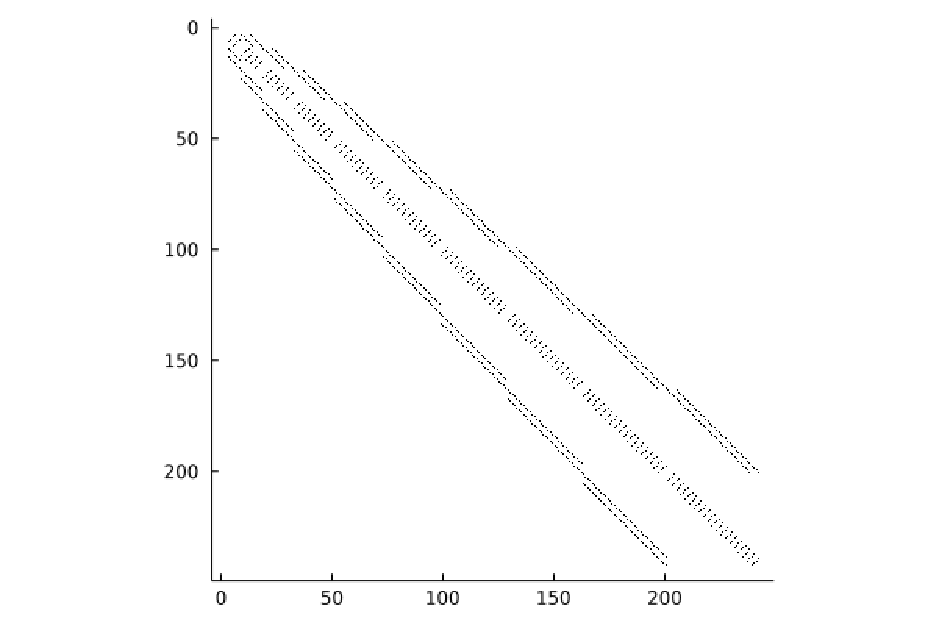
\includegraphics[scale=0.5]{spy-of-Jx-tangent}}
		\centering
		\caption{$\tangentjacobi_x$}
	\end{subfigure}\hfil % <-- added
	\begin{subfigure}{0.5\textwidth}
		\centerline{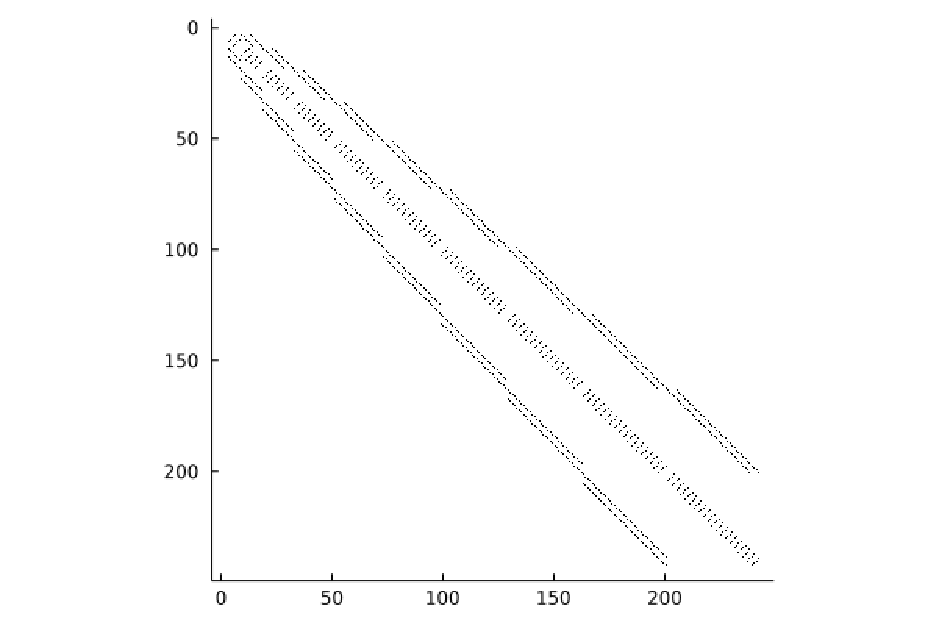
\includegraphics[scale=0.5]{spy-of-Jy-tangent}}
		\centering
		\caption{$\tangentjacobi_y$}
	\end{subfigure}\hfil % <-- added

	\medskip
	\begin{subfigure}{0.5\textwidth}
		\centerline{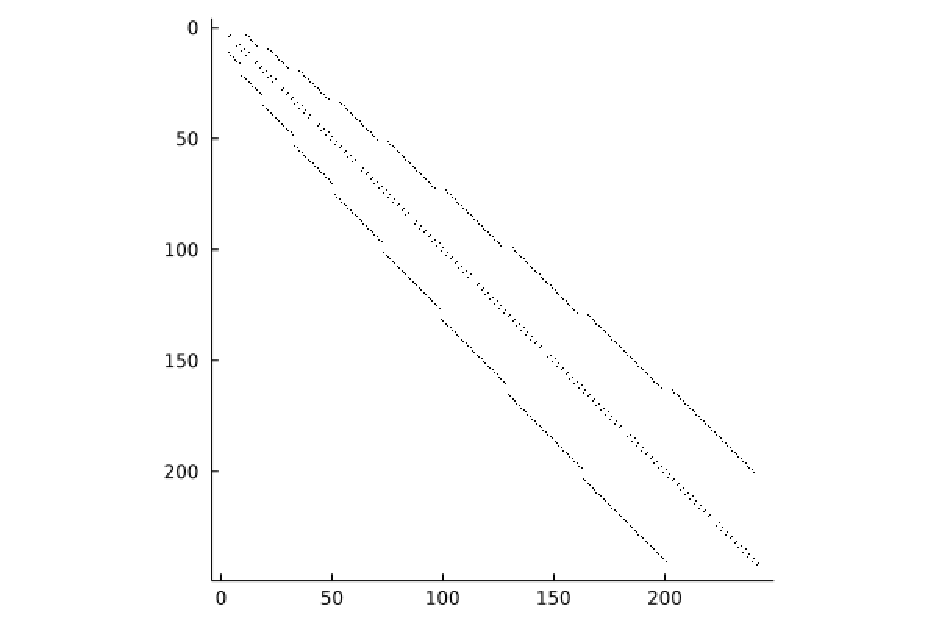
\includegraphics[scale=0.5]{spy-of-Jz-tangent}}
		\centering
		\caption{$\tangentjacobi_z$}
	\end{subfigure}\hfil % <-- added
	\caption{\enquote{Spy} plots of the Jacobi operator matrices for the vector spherical harmonic OP basis, showing their sparsity and structure, up to order $N=10$. These are block-tridiagonal, with sub-block bandwidths: (a) (4,4), (b) (4,4), (c) (2,2).}
	\label{fig:sh-spy-jacobi-tangent}
\end{figure}

The Jacobi matrices are then defined according to the matrices $\tangentjacobi_x, \tangentjacobi_y, \tangentjacobi_z$ satisfying
\bseqnnumber{
	\tangentjacobi_x \VSHvecfull(x,y,z) &= x \VSHvecfull(x,y,z) \nonumber \\
	\tangentjacobi_y \VSHvecfull(x,y,z) &= y \VSHvecfull(x,y,z) \label{eqn:tangentjacobimatdef} \\ 
	\tangentjacobi_z \VSHvecfull(x,y,z) &= z \VSHvecfull(x,y,z) \nonumber
}
for each $(x,y,z) \in \Omega$. The VSH Jacobi matrices are banded-block-banded due to the sparse relationships we obtain from \bsreflemma{lemma:VSHrecurrences}. Specifically, they each have block-bandwidths $(1,1)$:
\bseqn{
	\tangentjacobi_{x/y/z} &= 
		\begin{pmatrix}
			B_{x/y/z,0} & A_{x/y/z,0} & & & & \\
			C_{x/y/z,1} & B_{x/y/z,1} & A_{x/y/z,1} & & & \\
			& C_{x/y/z,2} & B_{x/y/z,2} & A_{x/y/z,2}  & & & \\
			& & C_{x/y/z,3} & \ddots & \ddots & \\
			& & & \ddots & \ddots & \ddots \\
		\end{pmatrix}.
}
Let \nomenclature[zerod]{$0_d$}{The zero matrix in $\R^{d \times d}$} $0_2 \in \R^{2\times2}$ be the $2\times2$ zero matrix. $\tangentjacobi_x$ has subblock-bandwidths $(4,4)$ since for $l \in \No$:
\bseqn{
	A_{x,l} &:= 
		\begin{pmatrix}
			\mathcal{A}_{l,-l,3} & 0_2 & \mathcal{A}_{l,-l,4} & & \\
			& \ddots & \ddots & \ddots & \\
			& & \mathcal{A}_{l,l,3} & 0_2 & \mathcal{A}_{l,l,4} \\
		\end{pmatrix} \in \R^{2(2l+1)\times2(2l+3)}, \\
	B_{x,l} &:= 
		\begin{pmatrix}
			0_2 & \mathcal{A}_{l,-l,6} & \\
			\mathcal{A}_{l,-l+1,5} & \ddots & \ddots \\
			& \ddots & \ddots & \mathcal{A}_{l,l-1,6} \\
			& & \mathcal{A}_{l,l,5} & 0_2
		\end{pmatrix}  \in \R^{2(2l+1)\times2(2l+1)}, \\
	C_{x,l} &:= 
		\begin{pmatrix}
			\mathcal{A}_{l,-l,2} & & & \\
			0_2 & \ddots & & \\
			\mathcal{A}_{l,-l+2,1} & \ddots & \ddots & \\
			& \ddots & \ddots & \mathcal{A}_{l,l-2,2} \\
			& & \ddots & 0_2 \\
			& & & \mathcal{A}_{l,l,1} \\
		\end{pmatrix} \in \R^{2(2l+1)\times2(2l-1)} \quad (l \ne 0),
}
where
\bseqn{
	\mathcal{A}_{l,m,j} := 
		\begin{pmatrix}
			A_{l,m,j} & 0 \\
			0 & A_{l,m,j}
		\end{pmatrix} \: \text{for } j = 1, 2, 3, 4, \quad
	\mathcal{A}_{l,m,j} := 
		\begin{pmatrix}
			0 & A_{l,m,j} \\
			- A_{l,m,j} & 0
		\end{pmatrix} \: \text{for } j = 5, 6.
}
Similarly, $\tangentjacobi_y$ also has subblock-bandwidths $(4,4)$ since for $l \in \No$:
\bseqn{
	A_{y,l} &:= 
		\begin{pmatrix}
			\mathcal{B}_{l,-l,3} & 0_2 & \mathcal{B}_{l,-l,4} & & \\
			& \ddots & \ddots & \ddots & \\
			& & \mathcal{B}_{l,l,3} & 0_2 & \mathcal{B}_{l,l,4} \\
		\end{pmatrix} \in \R^{2(2l+1)\times2(2l+3)}, \\
	B_{y,l} &:= 
		\begin{pmatrix}
			0_2 & \mathcal{B}_{l,-l,6} & \\
			\mathcal{B}_{l,-l+1,5} & \ddots & \ddots \\
			& \ddots & \ddots & \mathcal{B}_{l,l-1,6} \\
			& & \mathcal{B}_{l,l,5} & 0_2
		\end{pmatrix}  \in \R^{2(2l+1)\times2(2l+1)}, \\
	C_{y,l} &:= 
		\begin{pmatrix}
			\mathcal{B}_{l,-l,2} & & & \\
			0_2 & \ddots & & \\
			\mathcal{B}_{l,-l+2,1} & \ddots & \ddots & \\
			& \ddots & \ddots & \mathcal{B}_{l,l-2,2} \\
			& & \ddots & 0_2 \\
			& & & \mathcal{B}_{l,l,1} \\
		\end{pmatrix} \in \R^{2(2l+1)\times2(2l-1)} \quad (l \ne 0),
}
where
\bseqn{
	\mathcal{B}_{l,m,j} := 
		\begin{pmatrix}
			B_{l,m,j} & 0 \\
			0 & B_{l,m,j}
		\end{pmatrix} \: \text{for } j = 1, 2, 3, 4, \quad
	\mathcal{B}_{l,m,j} := 
		\begin{pmatrix}
			0 & B_{l,m,j} \\
			- B_{l,m,j} & 0
		\end{pmatrix} \: \text{for } j = 5, 6.
}
Finally, $\tangentjacobi_z$ has subblock-bandwidths $(2,2)$, as for $l \in \No$: 
\bseqn{
	A^z_l &:= 
		\begin{pmatrix}
			0 & 0 & \Gamma_{l,-l,2} \\
			& & & \Gamma_{l,-l,2} \\
			& & & & \ddots \\
			& & & & & \Gamma_{l,l,2} \\
			& & & & & & \Gamma_{l,l,2}& 0 & 0 \\
		\end{pmatrix} \in \R^{2(2l+1)\times2(2l+3)}, \\
	B^z_l &:= 
		\begin{pmatrix}
			0 & \Gamma_{l,-l,3} \\
			- \Gamma_{l,-l,3} & 0 \\
			& & \ddots \\
			& & & 0 & \Gamma_{l,l,3} \\
			& & & - \Gamma_{l,l,3} & 0 \\
		\end{pmatrix}  \in \R^{2(2l+1)\times2(2l+1)}, \\
	C^z_l &:= 
		\begin{pmatrix}
			0 \\
			0 \\
			\Gamma_{l,-l+1,1} \\
			& \Gamma_{l,-l+1,1} \\
			& & \ddots \\
			& & & \Gamma_{l,l-1,1} \\
			& & & & \Gamma_{l,l-1,1} \\
			& & & & 0 \\
			& & & & 0 \\
		\end{pmatrix} \in \R^{2(2l+1)\times2(2l-1)} \quad (l \ne 0).
}
The sparsity and structure of the Jacobi matrices for the VSHs as we have defined them can be seen visually in \bsreffig{fig:sh-spy-jacobi-tangent}.



\subsection{Three-term recurrence relation for $\VSHvecfull(x,y,z)$}\label{subsection:VSHrecurrence}

We can combine each system in \bsrefeqn{eqn:tangentjacobimatdef} into a block-tridiagonal system for any $(x,y,z) \in \Omega$:
\bseqn{
	\renewcommand\arraystretch{1.3}
	\begin{pmatrix}
		I_6 & & & \\
		B_1-G_1(x,y,z) & A_1 & & \\
		C_2 & B_2-G_2(x,y,z) & \quad A_3 \quad & \\
		& C_3 & B_3 - G_3(x,y,z)  & \ddots \\
		& & \ddots &\ddots
	\end{pmatrix}
	\VSHvecfull(x,y,z)
	=
	\begin{pmatrix}
		\VSHvecfull_1(x,y,z) \\ \vec{0} \\ \vec{0} \\ \vdots
	\end{pmatrix},
}
where we note that 
\bseqn{
	\VSHvecfull_{1}(x,y,z) := 
		\begin{pmatrix}
			\gradY_1^{-1}(x,y,z)^\top \\ \gradpY_1^{-1}(x,y,z)^\top \\ \gradY_1^{0}(x,y,z)^\top \\ \gradpY_1^{0}(x,y,z)^\top \\ \gradY_1^{1}(x,y,z)^\top \\ \gradpY_1^{1}(x,y,z)^\top \\
			\end{pmatrix}, 
}
can be calculated explicitly, and for each $l \in \N$,
\bseqnnumber{
	A_l &:= 
		\begin{pmatrix}
			A_{x,l} \\
			A_{y,l} \\
			A_{z,l}
		\end{pmatrix} \in \C^{6(2l+1)\times2(2l+3)}, \quad
	C_l := 
		\begin{pmatrix}
			C_{x,l} \\
			C_{y,l} \\
			C_{z,l}
		\end{pmatrix} \in \C^{6(2l+1)\times2(2l-1)} \quad (n \ne 0), \label{eqn:tangentclenshawmats1} \\
	B_l &:= 
		\begin{pmatrix}
			B_{x,l} \\
			B_{y,l} \\
			B_{z,l}
		\end{pmatrix} \in \C^{6(2l+1)\times2(2l+1)}, \quad
	G_n(x,y) := 
		\begin{pmatrix}
			x\idmat{2l+1} \\
			y\idmat{2l+1} \\
			z\idmat{2l+1}
		\end{pmatrix}  \in \C^{6(2l+1)\times2(2l+1)}. \label{eqn:tangentclenshawmats1}
}
Just like for the scalar case, for each $l = 0,1,2\dots$ let $\Dlt$ be any matrix that is a left inverse of $A_l$, i.e. such that $\Dlt A_l = \idmat{2(2l+3)}$. Multiplying our system by the preconditioner matrix that is given by the block diagonal matrix of the $\Dlt$'s, we obtain a lower triangular system \cite[p78]{dunkl2014orthogonal}, which can be expanded to obtain the recurrence:
\bseqn{
	\begin{cases}
		\VSHvecfull_{0}(x,y,z) := 0_{2,3} \\
		\VSHvecfull_{l+1}(x,y,z) = -\Dlt (B_l-G_l(x,y,z)) \VSHvecfull_l(x,y,z) - \Dlt C_l  \, \VSHvecfull_{l-1}(x,y,z), \quad l \in \N.
	\end{cases}
}
For $l \in \N$, we can set
\bseqnnumber{
	\Dlt = 
		\begin{pmatrix}
			& \vec{\eta}^\top_{0} & \\
			& \vec{\eta}^\top_{1} & \\
			0_{2(2l+1)} & 0_{2(2l+1)} & \quad \calD_l \quad \\
			& \vec{\eta}^\top_{2} & \\
			& \vec{\eta}^\top_{3} &
		\end{pmatrix} \in \R^{2(2l+3)\times6(2l+1)}, \label{eqn:VSHDltdef}
}
where $\calD_l \in \R^{2(2l+1) \times 2(2l+1)}$ is the matrix
\bseqn{
	\calD_l := 
		\begin{pmatrix}
			{1 \over \Gamma_{l,-l,2}} \\
			& {1 \over \Gamma_{l,-l,2}} \\
			& & \ddots \\
			& & & {1 \over \Gamma_{l,l,2}} \\
			& & & & {1 \over \Gamma_{l,l,2}}
		\end{pmatrix}
}
and where $\vec{\eta}_{0}, \vec{\eta}_{1}, \vec{\eta}_{2}, \vec{\eta}_{3} \in \R^{6(2l+1)}$ are vectors with entries given by 
\bseqn{
	\big(\vec{\eta}_{0}\big)_j &= 
		\begin{cases}
			{1 \over A_{l,-l,3}} & j = 1 \\
			{- \; A_{l,-l,4} \over A_{l,-l,3} \: \Gamma_{l,1-l,2}} & j = 4(2n+1) + 3 \\
			0 & o/w
		\end{cases}, \\
	\big(\vec{\eta}_{1}\big)_j &= 
		\begin{cases}
			\big(\vec{\eta}_{0}\big)_{j-1} & j = 2, 4(2l+1) + 4 \\
			0 & o/w
		\end{cases}, \\
	\big(\vec{\eta}_{2}\big)_j &= 
		\begin{cases}
			{1 \over A_{l,l,4}} & j = 2(2l+1) - 1 \\
			{- \; A_{l,l,3} \over A_{l,l,4} \: \Gamma_{l,l-1,2}} & j = 6(2l+1) - 3 \\
			0 & o/w
		\end{cases}, \\
	\big(\vec{\eta}_{3}\big)_j &= 
		\begin{cases}
			\big(\vec{\eta}_{2}\big)_{j-1} & j = 2(2l+1), 6(2l+1) - 2 \\
			0 & o/w
		\end{cases}.
}
%For $l = 0$ we can simply set
%\bseqnnumber{
%	D^T_0 = 
%		\begin{pmatrix}
%			\delta_1 & 0 & \delta_2 & 0 & 0 & 0 \\
%			0 & \delta_1 & 0 & \delta_2 & 0 & 0 \\
%			0 & 0 & 0 & 0 & {1 \over \Gamma_{0,0,2}} & 0 \\
%			0 & 0 & 0 & 0 & 0 & {1 \over \Gamma_{0,0,2}} \\
%			\delta_3 & 0 & \delta_4 & 0 & 0 & 0 \\
%			0 & \delta_3 & 0 & \delta_4 & 0 & 0
%		\end{pmatrix}. \label{eqn:VSHDzerotdef}
%}
%where
%\bseqn{
%	\delta_1 = {B_{0,0,4} \over A_{0,0,3} B_{0,0,4} - A_{0,0,4} B_{0,0,3}}, \quad \delta_2 = {- A_{0,0,4} \over A_{0,0,3} B_{0,0,4} - A_{0,0,4} B_{0,0,3}}, \\
%	\delta_3 = {B_{0,0,3} \over A_{0,0,4} B_{0,0,3} - A_{0,0,3} B_{0,0,4}}, \quad \delta_4 = {- A_{0,0,3} \over A_{0,0,4} B_{0,0,3} - A_{0,0,3} B_{0,0,4}}.
%}



\subsection{Computational aspects}

It will be useful to be able to describe the coefficients of a vector-valued function in the tangent bundle of $\Omega$ in multiple ways, and as such we will introduce some more notation for the \enquote{splitting} of the basis vectors into the two groups stemming from the gradient and perpendicular gradient directions. Let us explain what we mean by this. 

Define $\VSHvec, \VSHvecperp$ by
\bseqnnumber{
	\VSHvec &:= 
		\begin{pmatrix} 
			\VSHvec_0 \\ \VSHvec_1 \\ \vdots 
		\end{pmatrix}, \quad \text{where } \quad 
	\VSHvecl := 
		\begin{pmatrix} 
			(\gradY^{-l}_l)^\top \\ \vdots \\ (\gradY^{l}_l)^\top
		\end{pmatrix} \in \C^{(2l+1) \times 3} \quad \forall \: l \in \No, \label{eqn:VSHdef} \\
	\VSHvecperp &:= 
		\begin{pmatrix} 
			\VSHvecperp_0 \\ \VSHvecperp_1 \\ \vdots 
		\end{pmatrix}, \quad \text{where } \quad 
	\VSHvecperpl := 
		\begin{pmatrix} 
			(\gradpY^{-l}_l)^\top \\ \vdots \\ (\gradpY^{l}_l)^\top
		\end{pmatrix} \in \C^{(2l+1) \times 3} \quad \forall \: l \in \No. \label{eqn:VSHperpdef}
}
If $\uvec$ is a vector-valued function on the tangent bundle of $\Omega$, it will have the coefficients vectors $\uvec^c, \uvecc, \uveccperp$ for its expansion in the VSH basis up to order $N \in \N$, defined such that
\bseqn{
	\uvec(x,y,z) &\approx \VSHvecfull(x,y,z)^\top \: \uvec^c \\
	&\equiv \VSHvec(x,y,z)^\top \: \uvecc + \VSHvecperp(x,y,z)^\top \: \uveccperp \\
	&:=  \sum^N_{l=0} \sum^l_{m=-l} \big[u^{\gradY}_{l,m} \, \gradYlm(x,y,z)  + u^{\gradpY}_{l,m} \, \gradpYlm(x,y,z) \big].
}
Of course, just like for the scalar case, we can use transforms to compute the coefficients of such a known function, and further evaluate, and apply differential operators to, a function knowing just its coefficients.


\subsubsection{Obtaining coefficients}

As eluded to, we would like to be able to obtain the coefficients for the expansion of a vector valued function in the VSH basis up to a given degree, similar to how we approach the scalar case. To do this, we can use a vector spherical harmonic transform. The development of vector spherical harmonic transforms is well established \cite{swarztrauber1993vector}, and continues today (see \cite{gia2019favest}). 


\subsubsection{Function evaluation}
The Clenshaw algorithm presented in \bsrefsection{subsubsection:clenshaw} can also be used to evaluate a vector-valued function in the tangent bundle of $\Omega$, where the matrices $C_n, B_n, \Dnt, G_n(x,y,z)$ are all defined in \bsrefsection{subsection:VSHrecurrence}:
\bseqn{
	\quad &\text{1) } \text{Set } \vec{\xi}_{N+2} = \bold{0}, \: \vec{\xi}_{N+2} = \bold{0}. \\
	\quad &\text{2) } \text{For } n = N:-1:1 \\
	\quad & \quad \quad \quad \text{set } \vec{\xi}_{n}^\top = (\uvec^c_n)^\top - \vec{\xi}_{n+1}^\top \Dnt \big(B_n - G_n(x,y,z)\big) -  \vec{\xi}_{n+2}^\top D^\top_{n+1} C_{n+1} \\
	\quad &\text{3) } \text{Output: } \uvec(x,y,z) \approx \VSHvecfull_1(x,y,z)^\top \vec{\xi}_{1} \\
	&\quad \quad \quad \quad \quad \quad \quad \quad \quad = (\vec{\xi}_{1})_1 \gradY_1^{-1} + (\vec{\xi}_{1})_2 \gradpY_1^{-1} + (\vec{\xi}_{1})_3 \gradY_1^{0} \\
	&\quad \quad \quad \quad \quad \quad \quad \quad \quad \quad \quad + (\vec{\xi}_{1})_4 \gradpY_1^{0} + (\vec{\xi}_{1})_5 \gradY_1^{1} + (\vec{\xi}_{1})_6 \gradpY_1^{1}.
}
Here, at each iteration, the vector $\uvec^c_n$ is given by the merging of the two order $n$ subvector of $\uvec^c$:
\bseqn{
	\uvec^c_n := 
		\begin{pmatrix} 
			u^{\gradY}_{n,-n} \\
			u^{\gradpY}_{n,-n} \\
			\vdots \\
			u^{\gradY}_{n,n} \\
			u^{\gradpY}_{n,n} \\
		\end{pmatrix}.
}
Notice how the iteration also ends at $n=1$ (not $n=0$) here, since the VSHs for order $n=0$ are zero.


\subsection{Sparse partial differential operators}\label{section:SHdiffoperators}

The framework we have outlined for the spherical harmonics and the vector spherical harmonics allows us to easily and explicitly derive sparse operator matrices for partial differential operators such as the spherical gradient, divergence and Laplace--Beltrami, as well as other key operators found in examples such as the linearised shallow water equations. These operators will take coefficients of a function's expansion in either the SSH or VSH basis, to coefficients in either basis. 

Let $\uvec$ be a vector-valued function on the tangent bundle of $\Omega$ with coefficients vectors $\uvecc, \uveccperp$ for its expansion in the VSH basis up to order $N \in \N$, and let $f$ be a scalar function on $\Omega$ with coefficients vector $\fvecc$ for its expansion in the SSH basis also up to order $N$, i.e.
\bseqn{
	\uvec(x,y,z) &\approx \VSHvecfull(x,y,z)^\top \: \uvec^c \\
	&\equiv \VSHvec(x,y,z)^\top \: \uvecc + \VSHvecperp(x,y,z)^\top \: \uveccperp \\
	&:=  \sum^N_{l=0} \sum^l_{m=-l} \big[u^{\gradY}_{l,m} \, \gradYlm(x,y,z)  + u^{\gradpY}_{l,m} \, \gradpYlm(x,y,z) \big], \\
	f(x,y,z) &\approx \SHvec(x,y,z)^\top \: \fvecc :=  \sum^N_{l=0} \sum^l_{m=-l} f_{l,m} \, \Ylm(x,y,z).
}
In order to fully exploit the sparsity of the relationships and ensure we are using banded-block-banded operators, in problems where we have an interdependency of scalar and vector-valued functions it can be useful to \enquote{expand} the scalar function's coefficients vector $\fvecc$ to be the length of the vector-valued one $\uvec^c$, with zeros being inserted after each entry, i.e. define the \textit{expanded coefficients for a scalar function on $\Omega$ in the SH basis} by
\bseqn{
	\fveccexp :=
		\begin{pmatrix}
			\fveccexp_0 \\
			\vdots \\
			\fveccexp_N
		\end{pmatrix} \in \R^{2(N+1)^2}, \quad
	\fveccexp_l := 
		\begin{pmatrix}
			f_{l,-l} \\
			0 \\
			f_{l,-l+1} \\
			0 \\
			\vdots \\
		 	f_{l,l} \\
			0
		\end{pmatrix} \in \R^{4(l+1)}.
}
To help with the definitions of the operators we will discuss, let $\calE_s, \calE_v$ be (severely) rectangular matrices defined such that $\calE_s \fveccexp = \fvecc$ and $\calE_v \fvecc = \fveccexp$. We are now in a position to derive the sparse differential operators that can be applied to the functions $\uvec, f$.

\begin{definition}\label{def:SHoperators}
	We define the operator matrices $\calD, \tilde \calD, \calG, \tilde \calG, \calL$ according to:
\bseqn{
	\divergence \uvec(x,y,z) &= \SHvec(x,y,z)^\top \: \calD \: \uvecc, \\
	\divergence \uvec(x,y,z) &= \SHvec(x,y,z)^\top \: \calE_s \: \big(\tilde \calD \: \uvec^c), \\
	\gradS f(x,y,z) &= \VSHvec(x,y,z)^\top \: \calG \: \fvecc, \\
	\gradS f(x,y,z) &= \VSHvecfull(x,y,z)^\top \: \tilde \calG \: \fveccexp, \\
	\DeltaS f(x,y,z) &= \SHvec(x,y,z)^\top \: \calL \: \fvecc.
}
\end{definition}

\remark The operators $\tilde \calD, \tilde \calG$ would be used when vectors of the resulting length are required for the problem you are wishing to solve.

For clarity, we note that $\DeltaS$ is defined in \bsrefeqn{eqn:laplacebeltrami}, and the spherical gradient and divergence operators are given by
\bseqn{
	 \gradS &= \ppx{\varphi} + {1 \over \sinphi} \ppx{\theta}, \\
	 \divergence \uvec &= {1 \over \sinphi} \ppx{\varphi}\big( \sinphi u_\varphi \big) + {1 \over \sinphi} \ppx{\theta} u_\theta,
}
where $\uvec \equiv \phivec \: u_\varphi + \thetavec \: u_\theta$.

\begin{theorem}
	The operator matrices defined in \bsrefdef{def:SHoperators} are diagonal, and are given by:
\bseqn{
	\calD &\equiv \calL := 
		\begin{pmatrix}
			\calL_0 & & \\
			& \ddots & \\
			& & \calL_N
		\end{pmatrix} \in \R^{(N+1)^2 \times (N+1)^2}, \quad
	\tilde \calD = 
		\begin{pmatrix}
			\tilde \calD_0 & & \\
			& \ddots & \\
			& & \tilde \calD_N
		\end{pmatrix} \in \R^{2(N+1)^2 \times 2(N+1)^2}, \\
	\calG &= I_{(N+1)^2}, \quad
	\tilde \calG = 
		\begin{pmatrix}
			1 & & & & \\
			& 0 & & & \\
			& & \ddots & & \\
			& & & 1 & \\
			& & & & 0
		\end{pmatrix}  \in \R^{2(N+1)^2 \times 2(N+1)^2},
}
where
\bseqn{
	\calL_l := -l(l+1) \: I_{2l+1}, \quad
	\tilde \calD_l := \begin{pmatrix}
			-l(l+1) & & & & \\
			& 0 & & & \\
			& & \ddots & & \\
			& & & -l(l+1) & \\
			& & & & 0
		\end{pmatrix} \in \R^{2(2l+1) \times 2(2l+1)}.
}.
\end{theorem}

\begin{proof}
	The arguments for $\calG$ and $\tilde \calG$ are trivial by definition. The spherical harmonics, as the name eludes to, satisfy a harmonic relationship $\DeltaS \Ylm = \: l(l+1) \Ylm$ (see e.g. \cite{humi1987factorisation}). Thus, for the proof for $\calD$ and $\tilde \calD$, consider
\bseqn{
	\divergence \uvec &= \divergence \Big( \sum_{l=0}^N \sum_{m=-l}^{l} [ u^{\gradY}_{l,m} \gradYlm + u^{\gradpY}_{l,m} \gradpYlm ] \Big) \\
	&= \sum_{l=0}^N \sum_{m=-l}^{l} u^{\gradY}_{l,m} \: \DeltaS \Ylm \\
	&= \sum_{l=0}^N \sum_{m=-l}^{l} - u^{\gradY}_{l,m} \: l(l+1) \Ylm,
}
using the fact that $\divergence (\grad^\perp f )\equiv 0$ for any function $f$. We similarly have for $\calL$:
\bseqn{
	\DeltaS f &= \DeltaS \Big( \sum_{l=0}^N \sum_{m=-l}^{l} f_{l,m} \Ylm \Big) \\
	&= \sum_{l=0}^N \sum_{m=-l}^{l} f_{l,m} \: \DeltaS \Ylm \\
	&= \sum_{l=0}^N \sum_{m=-l}^{l} - f_{l,m} \: l(l+1) \Ylm.
}
\end{proof}


\section{Examples}\label{section:examples}

Now that we have our differential operators, let us apply them in some examples. 

\subsection{Heat equation}

\begin{figure}[t]
	\centering % <-- added
	\centerline{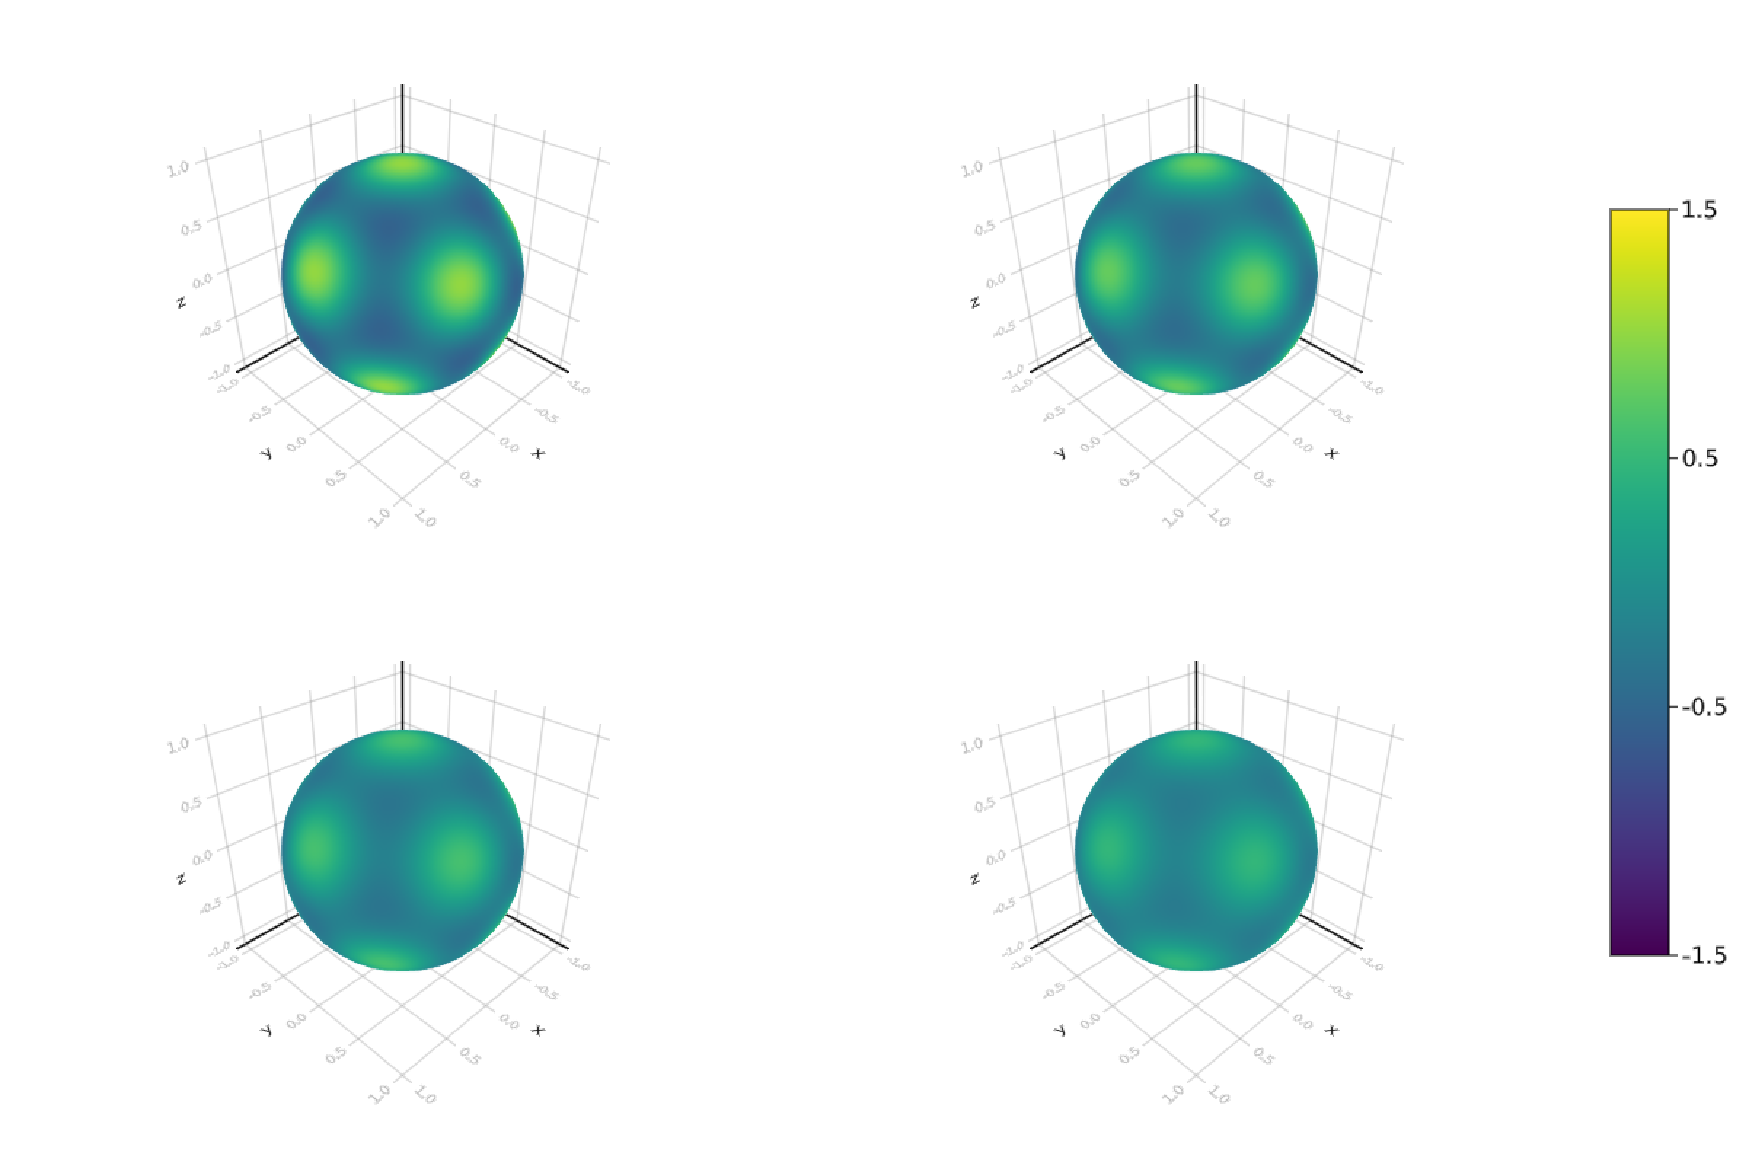
\includegraphics[scale=0.5]{heat-eqn-alpha-0p0238-dt=0p01-nsteps=100-2}}
	\caption{Four snapshots of the solution $u$ of the heat equation with $\alpha = 1/42$ and a step size of $\Delta t = 0.01$, solved using the BDF2 timestepping method. Top Left: Initial conditions (0 timesteps). Top Right: After 25 timesteps. Bottom Left: After 50 timesteps. Bottom Right: After 75 timesteps.}
	\label{fig:heateqn}
\end{figure}

To demonstrate proof of concept, we can apply the framework we have proposed to modelling the heat equation on the unit sphere. In doing so, we can demonstrate how our method allows us to expand and evaluate functions, and turn the differential equation into a matrix-vector problem at each timestep.

Let $u : \Omega \to \C$ represent the temperature at a point $(x,y,z)$ on the sphere and suppose that it is modelled by the equation
\bseqnnumber{
	\ppx{t}{u} = \alpha \DeltaS u \label{eqn:heateqn}
}
for some $\alpha \in \R$. A simple timestepping method we can use to iterate with is the BDF2 method \cite[�2.3]{iserles2009first}. Let $u_n$ for $n = 0, 1, 2, \dots$ be the solution at time $n \Delta t$ where $\Delta t$ is the timestep. The are timestepping method is \nomenclature[Delta t]{$\Delta t$}{A timestep for a simulation}
\bseqn{
	{u_1 - u_0 \over \Delta t} &= \alpha \DeltaS u_1 \\
	{3u_{n+1} - 4u_n + u_{n-1} \over 2\Delta t} &= \alpha \DeltaS u_{n+1}, \quad n = 1,2,\dots
}
$\iff$
\bseqn{
	[1 - \Delta t \alpha \DeltaS] u_1 -  &= u_0 \\
	[3 - 2\Delta t \alpha \DeltaS] u_{n+1} &= 4u_n - u_{n-1}, \quad n = 1,2,\dots.
}
Let us write this in coefficient space. Firstly, our coefficients vectors for the function $u$ we will denote $\uvec^c$ -- that is:
\bseqn{
	u(x,y,z) &\approx \SHvec(x,y,z)^\top \: \uvec^c.
}
Our system then becomes
\bseqn{
	[I - \Delta t \alpha \calL] \uvec^c_1 -  &= u_0 \\
	[3I - 2\Delta t \alpha \calL] \uvec^c_{n+1} &= 4\uvec^c_n - \uvec^c_{n-1}, \quad n = 1,2,\dots.
}
From here, it is clear that eat each timestep we simply have a fairly trivial linear system to solve, with the matrices $I - \Delta t \alpha \calL$, $3I - 2\Delta t \alpha \calL$ being banded-block-banded (in fact, simply diagonal here). We demonstrate this theory in \bsreffig{fig:heateqn}, where we see four snapshots of the solution to the heat equation in \bsrefeqn{eqn:heateqn} on the unit sphere with our order $N$ set large enough (here, $N=20$). We set $\alpha = {1 \over 42}$ and a step size of $\Delta t = 0.01$, and take the initial condition for the heat $u$ to be a \enquote{football function}\footnote{These initial conditions are taken from an example found at https://www.chebfun.org/examples/sphere/SphereHeatConduction.html} -- that is we take
\bseqn{
	u_0 := Y_6^0 + \sqrt{14 \over 11} Y_6^6.
}
The snapshots of the solution $u$ in \bsreffig{fig:heateqn} are taken of the initial conditions, plus after $25$, $50$ and $75$ timesteps respectively.


\subsection{Linearised shallow water equations}

\begin{figure}[t]
	\centering % <-- added
	\centerline{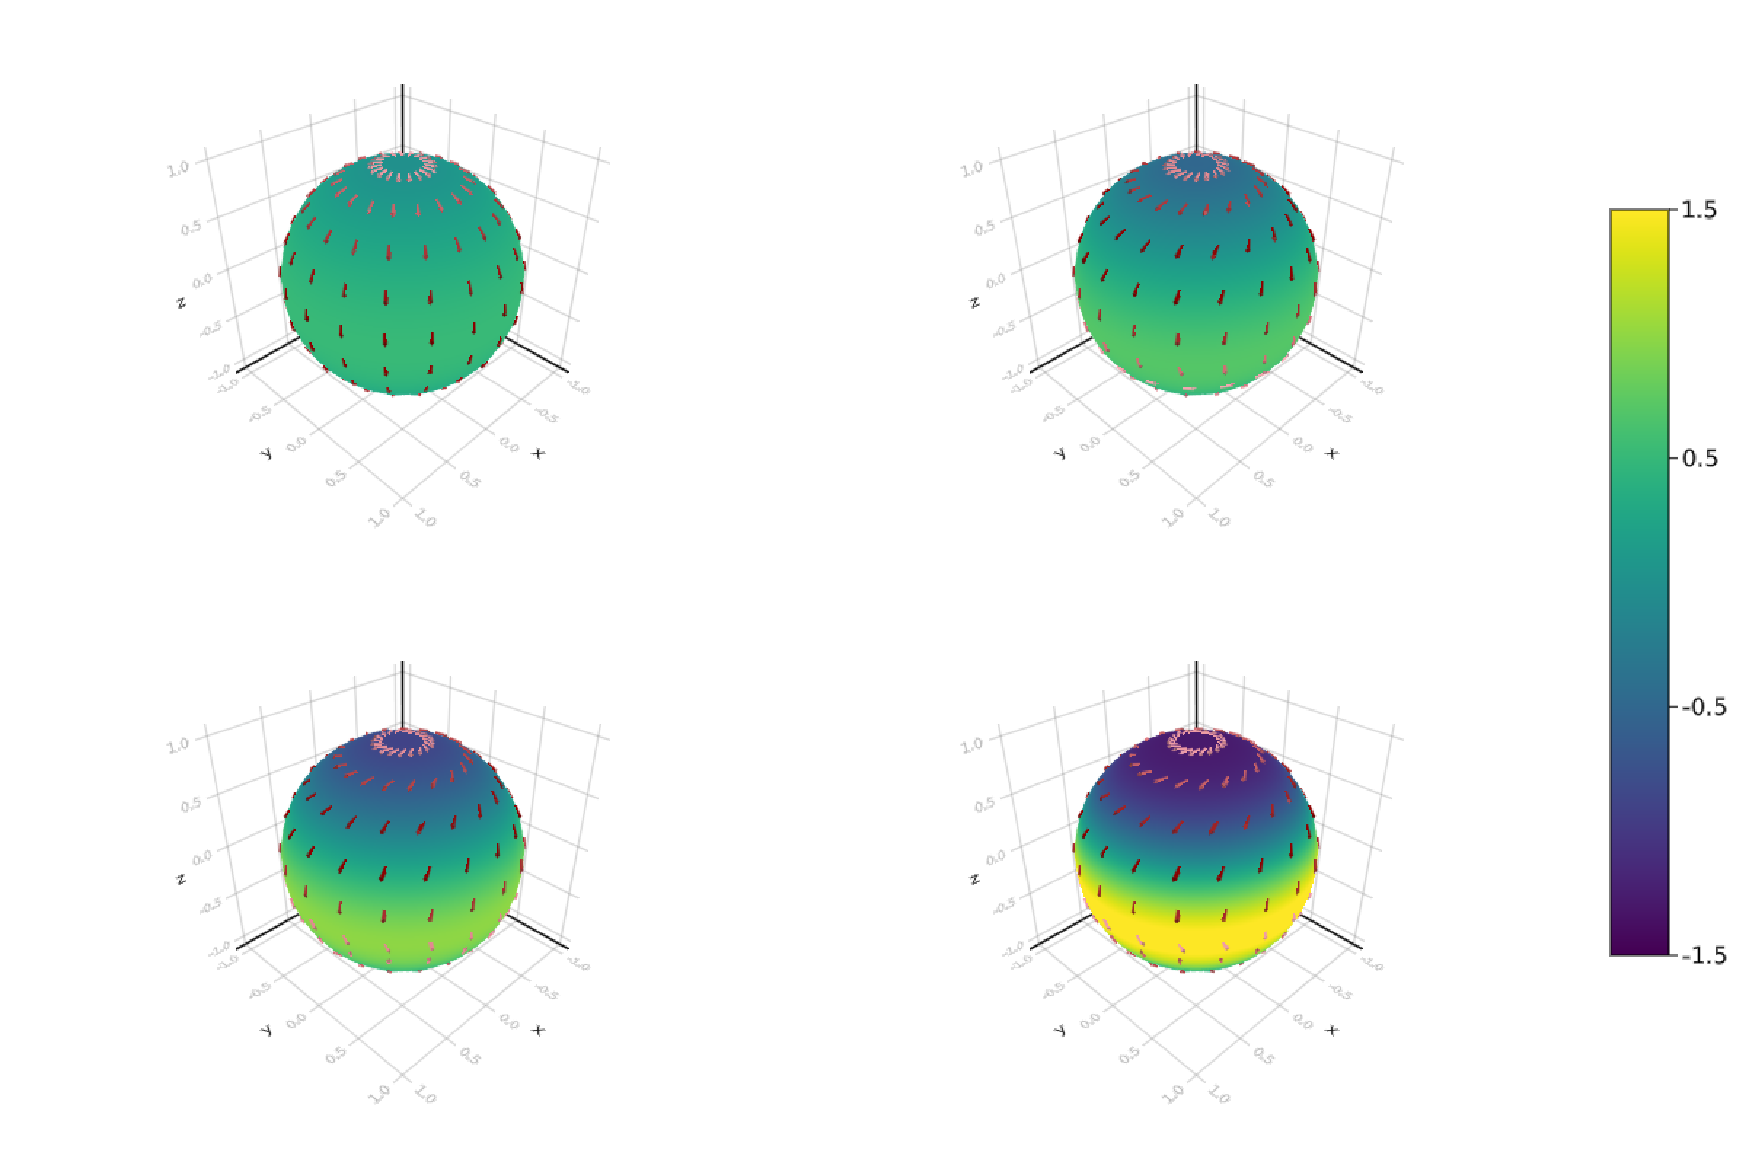
\includegraphics[scale=0.5]{linear-swe-H=1-dt=0p01-nsteps=100-arrows-2}}
	\caption{Four snapshots of the solution for the height $h$ (surface colour) and the wave velocity $u$ (red arrows) of the linearised shallow water equations with $\rotrate = \calH = 1$ and a step size of $\Delta t = 0.01$, solved using the backwards Euler timestepping method (BDF1). The initial conditions are given in \bsrefeqn{eqn:sweics}. Top Left: Initial conditions (0 timesteps). Top Right: After 50 timesteps. Bottom Left: After 75 timesteps. Bottom Right: After 100 timesteps.}
	\label{fig:swe}
\end{figure}

The linearised shallow water equations allow us to showcase more of the differential operators that we defined in \bsrefdef{def:SHoperators} (namely the divergence and gradient operators) and demonstrate how the natural sparsity that our framework brings to the problem leads to a simple sparse linear system to solve.

Let $\uvec(x,y,z)$ be the tangential velocity of a flow and $h(x,y,z)$ be the height deviation of the flow from some constant reference height $\calH$. Define $\rvec$ as the unit outward normal vector at the point on the sphere $(x,y,z)$, so that
\bseqn{
	\rvec = \begin{pmatrix} x \\ y \\ z \end{pmatrix}.
}
The linear SWEs are
\bseqnnumber{
	\begin{cases}
		\pfpx{t}{\uvec} + f \rvec \times \uvec - \gradS h = \mathbf{0} \\
		\pfpx{t}{h} + \calH \gradS \cdot \uvec = 0
	\end{cases} \label{eqn:swe}
}
where $f = 2 \rotrate \cos(\varphi) =  2 \rotrate z$ is the Coriolis parameter\footnote{Normally, the Coriolis parameter is expressed in terms of the latitude: $\text{latitude} = {\pi \over 2} - \varphi$}, and $\rotrate$ is the rotation rate of the sphere surface (that is, the amount the body rotates per unit time)\footnote{On a full scale Earth, the rotation rate is $\rotrate = 7.2921 � 10^{-5}$ rad s$^{-1}$.}.

A keen eye may notice that -- while we have operators for the multiplication by $z$, the spherical gradient and divergence -- we require one more operator not yet defined for the unit vector cross product $\rvec \times \uvec$.
\begin{definition}\label{def:unitveccrossproduct}
	Define the operator matrix $\calR$ according to:
\bseqn{
	\rvec(x,y,z) \times \uvec(x,y,z) &= \VSHvecfull(x,y,z)^\top \: \calR \uvec^c.
}
\end{definition}
\begin{lemma}
	The operator $\calR$ defined in \bsrefdef{def:unitveccrossproduct} is sparse with banded-block-banded structure. More specifically, $\calR$ has block-bandwidths $(0,0)$, and sub-block-bandwidths $(1,1)$ (i.e. is tridiagonal).
\end{lemma}
\begin{proof}
	Using the relations that $\gradYlm = \gradS \Ylm$ and $\gradpYlm = \rvec \times \gradS \Ylm$ for each $l \in \N$, $m \in \Z$ s.t. $-l \le m \le l$, we have that:
\bseqn{
	\rvec \times \bold{u} &= \rvec \times \sum_{l=0}^{N} \sum_{m=-l}^{l} [ u^{\gradY}_{l,m} \gradYlm + u^{\gradpY}_{l,m} \gradpYlm ] \\
	&= \sum_{l=0}^{N} \sum_{m=-l}^{l} [ u^{\gradY}_{l,m} \rvec \times \gradYlm + u^{\gradpY}_{l,m} \rvec \times ( \rvec \times \gradYlm ) ] \\
	&= \sum_{l=0}^{N} \sum_{m=-l}^{l} [ u^{\gradY}_{l,m} \: \gradpYlm - u^{\gradpY}_{l,m} \: \gradYlm ) ].
}
We can then write down the operator $\calR$ as follows:
\bseqn{
	\calR &=
		\begin{pmatrix}
			R & & & \\
			& R & & \\
			& & & \ddots
		\end{pmatrix} \in \R^{2(N+1)^2 \times 2(N+1)^2},
}
where the blocks $R$ are simply given by
\bseqn{
	R &:= 
		\begin{pmatrix}
			0 & -1 \\
			1 & 0
		\end{pmatrix} \in \R^{2\times2}.
}
\end{proof}

For simplicity, we will implement a backward Euler timestepping method to solve the linear SWEs with timestep $\Delta t$. Of course, other timestepping methods are equally implementable (for example, the method used in the IFS model that ECMWF uses is a semi-implicit, semi-Lagrangian (SISL) timestepping method \cite{diamantakisecmwf}), but we simplify things here to show proof of concept. Using $\uvec_n, h_n$ to represent the solution at time $n\Delta t$:
\bseqn{
	\uvec_{n+1} &= \uvec_{n} + \Delta t \: (\gradS h_{n+1} - f \rvec \times \uvec_{n+1}) \\
	h_{n+1} &= h_n - \Delta t \: \calH \gradS \cdot \uvec_{n+1}
}
Let us write this in coefficient space. Firstly, our coefficients vectors for the functions $\uvec, h$ we will denote $\uvec^c, \vec{h}^c$ -- that is:
\bseqn{
	\uvec(x,y,z) &\approx \VSHvecfull(x,y,z)^\top \: \uvec^c \\
	h(x,y,z) &\approx \SHvec(x,y,z)^\top \: \vec{h}^c.
}
As eluded to earlier, we will \enquote{extend} the scalar function's coefficients vector, writing $\tilde{\vec{h}}^c = \calE_v \vec{h}^c$, as described in \bsrefsection{section:SHdiffoperators}. Thus, our system can be written as a matrix-vector system:
\bseqn{
	\uvec^c_{n+1} &= \uvec^c_n + \Delta t \: (\tilde \calG \tilde{\vec{h}}^c_{n+1} - 2 \rotrate \tangentjacobi_z \calR \uvec^c_{n+1}) \\
	\tilde{\vec{h}}^c_{n+1} &= \tilde{\vec{h}}^c_n - \Delta t \: \calH \tilde \calD \uvec^c_{n+1}
}
$\iff$
\bseqn{
	\uvec^c_{n+1} &= \uvec^c_n + \Delta t \: (\tilde \calG \tilde{\vec{h}}^c_{n} - \Delta t \: \calH \tilde \calG \tilde \calD \uvecc_{n+1} - 2 \rotrate \tangentjacobi_z \calR \uvec^c_{n+1}) \\
	\tilde{\vec{h}}^c_{n+1} &= \tilde{\vec{h}}^c_n - \Delta t \: \calH \tilde \calD \uvec^c_{n+1}
}
$\iff$
\bseqn{
	\Big[ I + \Delta t^2 \calH \tilde \calG \tilde \calD + 2 \rotrate \Delta t \: \tangentjacobi_z \calR \Big] \: \uvec^c_{n+1} &= \uvec^c_n + \Delta t \tilde \calG \tilde{\vec{h}}^c_{n} \\
	\tilde{\vec{h}}^c_{n+1} &= \tilde{\vec{h}}^c_n - \Delta t \: \calH \tilde \calD \uvec^c_{n+1}.
}
Here, it is clear that the matrix $I + \Delta t^2 \calH \tilde \calG \tilde \calD + 2 \rotrate \Delta t \: \tangentjacobi_z \calR$ is sparse with banded-block-banded structure, and hence this system will be efficient to solve. Doing so at each iteration provides us with the coefficients vectors $\uvec^c_{n+1}, \tilde{\vec{h}}^c_{n+1}$ if we know $\uvec^c_{n}, \tilde{\vec{h}}^c_{n}$. Of course, when evaluating the function $h$, we can simply gather back the coefficients vector $\vec{h}^c$ by $\vec{h}^c = \calE_s \tilde{\vec{h}}^c$.

As a demonstration, in \bsreffig{fig:swe} we see four snapshots of the solution to the system in \bsrefeqn{eqn:swe} on the unit sphere, with $\rotrate = \calH = 1$ and initial conditions given by
\bseqnnumber{
	\uvec_0 := \phivec \mu \sinphi, \quad h_0 := \mu \sin^2\varphi, \label{eqn:sweics}
}
where $\mu = {\pi \over 6}$, with the solution order $N$ set large enough (here, $N=20$). This example is very similar to \enquote{test case 2} in the well-known standard test set for shallow water equations in spherical geometries \cite{williamson1992standard}. The snapshots of the wave height $h$ are taken of the initial conditions, plus after $50$, $75$ and $100$ timesteps respectively, using a step size of $\Delta t = 0.01$.


\section{Conclusion}

Spherical harmonics have been widely used to solve PDEs, in particular a spherical harmonics approach is used as part of the Integrated Forecasting System (IFS) that ECMWF uses for their forecasts. In this chapter, we have chosen to view the spherical harmonics as orthogonal (in fact orthonormal) polynomials in $x$, $y$ and $z$ in order to illustrate and understand more about how the framework presented here for using multivariate OPs in a spectral method translate to the sphere. We have derived the entries of \textit{Jacobi matrices} that represent multiplication by the coordinates, showing how they are \textit{banded-block-banded} in structure. We have set out how one can find coefficients for the expansion of a function in the spherical harmonics basis using established transforms, and how one can evaluate a function given its coefficients vector using a multidimensional version of the Clenshaw algorithm. We extended our framework to include the \textit{tangent bundle} of the sphere -- that is, the space of vectors orthogonal to the unit outward normal for each point on the sphere -- where we can use the \textit{vector spherical harmonics} as vector-valued orthogonal polynomials to be a basis, demonstrating how similar such Jacobi matrices, function expansion and evaluation can be derived. Further, by exploiting the natural sparsity of the relationships between the OPs in the bases, we have shown how matrices for differential and other operators will be sparse and banded-block-banded in structure too. In fact, for the spherical harmonics, these are simply diagonal. Finally, we presented a couple of simple examples of how one can put this all into practice, namely solving the heat equation and the linearised shallow water equations on the unit sphere.














  